\documentclass[UTF8,12pt]{ctexart}
\usepackage{amsmath,amssymb,geometry,bm,graphicx,fontspec,amssymb,amsthm}
\usepackage[mathscr]{euscript}
\usepackage{array}

\usepackage[colorlinks,
linkcolor=black,
anchorcolor=blue,
citecolor=green
]{hyperref} % 目录中的超链接

\usepackage{tikz}
\usetikzlibrary{calc}
\usetikzlibrary{shapes.geometric}
% Node styles
\tikzset{
	% Two node styles for game trees: solid and hollow
	solid node/.style={circle,draw,inner sep=1.5,fill=black},
	hollow node/.style={circle,draw,inner sep=1.5}
}

\newtheorem{Def}{定义}[section]
\newtheorem{Theo}{定理}[section]
\newtheorem{Lemm}{引理}[section]
\newtheorem{Prop}{命题}[section]
\newtheorem{Axiom}{Axiom}
\newtheorem{Req}{要求}[section]

\numberwithin{equation}{section} % 按章节进行排序与编号
\numberwithin{figure}{section}
\numberwithin{table}{section}

\usepackage{draftwatermark} % 所有页加水印
\SetWatermarkText{EconNerd} % 设置水印内容
\SetWatermarkLightness{0.99} % 设置水印透明度 0-1
\SetWatermarkScale{1} % 设置水印大小    

\title{博弈论} % 文档相关信息
\author{EconNerd}
\date{\today}
\geometry{scale=0.8}

\begin{document}
	\maketitle
	\tableofcontents
	
	\newpage
	
	\part{基础}
	\section{如何进行理性选择}
	在本章我们首先考虑一个最简单的选择问题。选择问题是我们分析更复杂博弈的一个基础。
	
	一个最简单的决策问题需要包含三个要素。动作(action)、结果(outcome)以及对于不同结果的偏好关系(preferences)。偏好关系用$\succsim$来表示。$x \succsim y$表示$x$至少和$y$一样好。通过这个偏好关系我们可以定义严格的偏好关系$\succ$和无差异的关系$\sim$。
	
	在后面的分析中,我们会进行一些假设。即我们假设偏好关系是理性的偏好关系(rational preference relation)。这意味着这个关系是完备的,且具有传递性。
	
	对于偏好关系进行分析比较复杂,我们采用一个payoff函数来表示偏好关系,并基于payoff函数进行分析。
	
	首先的问题就是,对于一个偏好关系,是否一定存在着一个payoff函数来表示他呢?答案是肯定的。
	
	在有了payoff函数后,我们可以基于函数值来构建决策树,使得分析的过程简洁明了。
	
	\subsection{理性分析范式}
	除了对于偏好关系进行假设,我们分析的另一个基础假设就是理性人假设,Homo economicus。一般来说可以表示为如下形式
	
	\paragraph{理性选择假设}
	决策者知道如下的信息
	\begin{enumerate}
		\item 所有可能的行动$A$
		
		\item 所有可能的结果$X$
		
		\item 行动是如何影响结果的
		
		\item 自身对于不同结果的偏好关系
	\end{enumerate}

	\subsection{不确定性}
	对于一个最简单的决策问题,我们可以直接最大化payoff来解决决策问题。但是问题中可能存在着不确定性。
	
	即当agent选择了一个动作后,与这个动作所关联的结果是随机的。那么我们就可以用随机变量来描述这个结果。这个随机变量可以是离散的、也可以是连续的。
	
	我们用彩票的视角来看待这个随机变量。当我们给出一个彩票时,我们实际上是给出了所有可能的结果出现的概率,以及所有结果带来的payoff。
	
	在这样的描述之下,我们之前分析的确定性的情况其实就是随机情况的一种简化版本。
	
	那么对于这种随机的情况,不同于在确定情况下,agent直接通过payoff来确定决策。在这里,agent通过payoff的期望值来确定决策,即冯诺依曼-摩根斯坦效用函数类似形式的函数。
	
	离散情况下就是有限项的和、连续情况下就是一个定积分。
	
	在这种情况下,我们的payoff函数和之前确定情况下的payoff函数存在着区别。之前的payoff函数的值并不重要,只要这个函数表示了偏好关系就可以。但是在随机的情况下,payoff函数的值也十分重要,因为这个值可以看作是不同结果的权重。
	
	而不同的payoff函数还表示了不同的风险态度。风险中性(risk neutral)、风险厌恶(risk averse)、风险偏好(risk loving)。
	
	在不确定的情况下,我们的分析都是以最大化期望payoff来执行的。
	
	\subsection{时间}
	当涉及到时间时,即在决策问题中存在多个阶段。这时候有两个需要注意的点。
	
	第一个点就是如何求解这样的多个阶段的决策问题。我们运用逆向归纳(backward induction)。首先求解最后的节点上agent理性的决策是什么,然后根据最后节点上的决策将我们的决策树进行简化,然后向上求解。直到最后求解到根节点。
	
	第二个点就是折现问题,不同时间段上的payoff可能还需要考虑折现的问题。
	
	\subsection{博弈}
	以上就是我们分析的一个最简单的问题,即单个agent的决策问题。当存在多个agent互相影响的决策问题时,我们称之为博弈(game)。
	
	一般来说,存在着四种类型的博弈。静态完全信息、静态不完全信息、动态完全信息、动态不完全信息。
	
	其中静态意味着所有的agent是同时做出行为的,而动态则意味着不同agent选择行为时存在着先后顺序。
	
	完全信息意味着所有和博弈相关的信息都是共同知识(common knowledge),即所有者agent都知道这些信息,且他们也知道其他的agent都知道这些信息。不完全信息则意味着某些agent有着自己的私人信息。
	
	后续我们会对这四种不同类型的博弈进行分析,并探求如何求解这些博弈。
	
	\newpage
	
	\part{完全信息静态博弈}
	在之前我们已经定义了完全信息和静态博弈。但是在这个类型中还可以细分,就是agent是如何进行行为的选择的。如果agent是进行确定性选择的,那么这个博弈就是\textbf{纯策略}的;如果agent是进行包含不确定的选择的(即以某个概率分布来选择行动),那么这个博弈就是\textbf{混合策略}的。
	
	我们会对这两种博弈分别进行研究,首先我们来考虑纯策略的博弈
	
	\section{纯策略博弈}
	首先我们要定义一下什么是纯策略
	\begin{Def}
		player i的纯策略就是一组确定性的行动。player i的所有纯策略的组合表示为$S_i$。一个纯策略的profile表示为$s = (s_1,s_2,\cdots,s_n),s_i \in S_i,\forall i = 1,2,\cdots,n$。表示为所有player选择的策略的组合。且$s = (s_1,s_2,\cdots,s_n) \in S_1 \times S_2 \times \cdots \times S_n$
	\end{Def}
	
	策略(strategy)这个概念也十分重要,一般来说可以把策略看成是一系列有时序的动作组合。
	
	有了这些概念,我们可以给出一个博弈形式化的定义。
	\begin{Def}
		一个博弈的Normal-Form包含以下的三个部分
		\begin{enumerate}
			\item 有限的player集合,$N = \{1,2,\cdots,n\}$
			
			\item 所有player纯策略的集合,$\{S_1,S_2,\cdots,S_n\}$
			
			\item 一组所有player的payoff函数的集合$\{v_1,v_2,\cdots,v_n\}$,且函数定义为$v_i:S_1 \times S_2 \times \cdots \times S_n \rightarrow \mathbb{R},\forall i \in N$
		\end{enumerate}
	\end{Def}
	
	实际上我们就可以用一个三元组$<N,\{S_i\}_{i=1}^n,\{v_i(\cdot)\}_{i=1}^n>$来表示一个博弈。对于两个player和有限策略的情况,我们也可以用矩阵来表示这样的博弈。
	
	\subsection{solution concept}
	
	当我们有了一个博弈后,很自然的就是想要找到在这个博弈中\textbf{更加可能出现的结果}。我们借助solution concept可以完成这个目标。solution concept是一种方法论,来在所有可能的结果中找出那些更加可能发生的结果。本质上就是我们会对player设定一些目标,并假定他们在追求这些目标,最终得到一个博弈的解。
	
	例如对于囚徒困境这个博弈,我们可以假设所有的囚徒都追求严格占优的策略,即这个策略要使得对方无论怎么选择,自己都有好的结果。那么这样我们就可以求出一个博弈的解。
	
	所以可以看到的一点是,如果我们设定不同的标准,我们也会得到不同的均衡。因此设定怎么样的标准就是一个重要的问题,一般来说有着三个标准。existence, uniqueness, invariance。
	\begin{enumerate}
		\item existence要求你设定的标准应该使得博弈存在着解。
		
		\item uniqueness则要求你设定的标准应该使得博弈的解不要过多。可以看到这两个指标使得我们在设定标准时有着权衡取舍。
		
		\item invariance则要求当我们对博弈的payoff进行了一个微小的改变后,不会改变博弈的解。
	\end{enumerate}
	
	除了solution concept存在着评判标准。当我们求出一个博弈的解后,我们还可以运用帕累托的标准来判定这个解是否是最优的。
	
	接下来我们考虑不同的solution concept,并且根据我们之前的三个标准来分析不同的solution concept。需要注意的是,虽然有着多种的solution concept,但是纳什均衡是我们求解的重点。
	
	\subsection{占优策略均衡}
	本质上,我们在考虑不同的solution concept时,我们就是在考虑或者说假定player执行了什么样的策略。
	
	首先我们考虑什么是严格占优?我们给出如下的定义
	\begin{Def}
		令$s_i,s'_i \in S$为player i所有可能的策略,当
		\begin{equation}
			v_i(s_i,s_{-i}) > v_i(s'_i,s_{-i}),\forall s_{-i} \in S_{-i}
		\end{equation}
		则我们称$s_i$为严格占优于$s'_i$
	\end{Def}
	
	同样的,我们也可以得到一个策略被劣势于另一个策略的定义。当一个策略对于所有其他可能的策略都是占优时,这个策略就是严格占优策略。我们给出如下的定义
	\begin{Def}
		令$s_i,s'_i \in S$为player i所有可能的策略,当
		\begin{equation}
			v_i(s_i,s_{-i}) > v_i(s'_i,s_{-i}),\forall s_{-i} \in S_{-i},\forall s'_i \in S  
		\end{equation}
		则我们称$s_i$为严格占优策略
	\end{Def}
	
	那么在占优策略的均衡中,我们对player做出他们都是理性的假设。这意味着所有player都不会选择劣势的策略。
	
	在这样的假设下,我们就可以给出严格占优策略均衡的定义
	\begin{Def}
		如果$s^D_i \in S_i,\forall i \in N$是一个严格占优策略,那么我们就说这些策略组合成的profile \ $s^D \in S$就是一个严格占优策略均衡(strict dominant strategy equilibrium)。
	\end{Def}
	
	关于严格占优策略的唯一性,我们有如下命题
	\begin{Prop}
		如果一个博弈$\Gamma = <N,\{S_i\}_{i=1}^n,\{v_i\}_{i=1}^n>$有着严格占优策略均衡$s^D$,那么这个均衡是唯一的。
	\end{Prop}
	
	接下来我们从三个标准来考虑一下这个solution concept。
	
	就existence来说,博弈可能并不会存在严格占优策略均衡。在uniqueness方面,如果一个博弈存在严格占优策略均衡,那么这个博弈一定只有一个严格占优策略。在invariance方面,对payoff的改变并不会影响这个解的情况。
	
	\subsection{重复剔除严格劣策略}
	在这个solution concept中,我们除了假定所有player都是理性的,我们还假设所有player都是理性的是一个共同知识,即所有player都知道其他player是理性的。
	
	在添加了假设后,整个分析过程又会产生不同。既然所有player的理性是共同知识,那么我们就可以剔除那些严格劣势的策略,并不断迭代这个过程,并将最后剩下的策略作为博弈的解。
	
	这个过程也叫做重复剔除严格劣策略(iterated elimination of strictly
	dominated strategies,IESDS)
	
	IESDS可以运用于所有的博弈,但是他产出的解并不一定是唯一的,且有些时候并不会剔除任何可能性。
	
	但是IESDS和严格占优均衡之间存在着联系,如果一个博弈有着严格占优均衡,那么这个均衡一定是唯一的IESDS。
	
	\subsection{可理性化策略}
	在之前的两次分析中,我们的方法都是剔除那些player不可能选择的策略。在这里我们考虑player可能选择的策略。很显然player会根据其他player选择的策略来进行选择,对于其他参与者的任何选择,player都有一个best response。
	
	那么如何确定其他的player做的什么选择呢?这实际上就和belief有关,belief可以是其他player的任何策略选择。引入了belief后,对于任意的belief,我们的player都有对应的best response,即一个策略的组合。这种对应并不是一种函数。
	
	我们可以用best response来和IESDS一样剔除那些永远不可能是best response的策略,并最终得到最后的解。这个也叫做可理性化。
	
	就existence, uniqueness来说,可理性化和IESDS是相同的。实际上这两种方法十分的类似。
	
	\subsection{纳什均衡}
	之前介绍了三种不同的solution concept。在这一节,我们会引入更加严格的假设,从而介绍一种非常重要的solution concept,纳什均衡。
	
	在之前的solution concept中,我们引入了belief和best response来简化博弈,从而得到博弈的解。但是我们并没有考虑player的belief是否是正确的。
	
	因此为了得到纳什均衡,我们对player做出以下两个假设
	\begin{enumerate}
		\item 每个player都对针对他的belief实施best response
		
		\item 每个player对于其他人的belief都是正确的
	\end{enumerate}
	第一个假设只是对于之前solution concept的重复,第二个假设才是使得纳什均衡和其他的solution concept产生本质区别的假设。这实际上是一个更加严格的假设,因为他要求所有的player都能正确地预测其他player的行为。
	
	由此我们给出纯策略中的纳什均衡的定义
	\begin{Def}
		一个纯策略的profile \ $s^* = (s^*_1,s^*_2,\cdots,s^*_n) \in S$是一个纳什均衡,当且仅当对于任意的$i \in N$,$s^*_i$都是$s^*_{-i}$的best response。也就是说
		\begin{equation}
			v_i(s^*_i,s^*_{-i}) \geqslant v_i(s'_i,s^*_{-i}) ,\forall s'_i \in S_i,\forall i \in N			
		\end{equation}
	\end{Def}
	
	可以看到,纳什均衡在之前的solution concept中添加了更多的假设,实际上纳什均衡和之前的三种solution concept也存在着关系。
	\begin{Prop}
		对于一个策略的profile$s^* = (s^*_1,s^*_2,\cdots,s^*_n)$如果$s^*$满足以下任意一个条件
		\begin{enumerate}
			\item $s^*$是一个严格占优均衡
			
			\item $s^*$是ELSDS唯一的解
			
			\item $s^*$是唯一的可理性化的profile
		\end{enumerate}
		那么$s^*$就是唯一的纳什均衡
	\end{Prop}
	
	在使用矩阵分析博弈时,我们可以在矩阵中标出每个player的best response,这样我们就可以很容易地求出纳什均衡。
	
	在用之前的三种标准来分析纳什均衡时,我们可以很容易地看到,一个博弈中可能并不只存在一个纳什均衡,但是博弈中总会存在纳什均衡,虽然并不一定是纯策略的纳什均衡。解纳什均衡的结果总是比IESDS更加精炼。且和之前的三个solution concept一样,我们得到的解并不一定时帕累托最优的,我们需要根据具体的博弈进行分析。
	
	
	\section{混合策略}
	在之前的纯策略中,我们的player都是选择确定的行动。在这里我们引入混合策略,即player可以以随机的方式选择行动。
	
	因此我们在纯策略的基础上给出混合策略的定义。
	\begin{Def}
		令$S_i = \{s_{i1},s_{i2},\cdots,s_{im}\}$为player i的有限策略集合。我们定义$\Delta S_i$为$S_i$的simplex,为$S_i$上所有可能的概率分布的集合。由此我们定义混合策略$\sigma_i \in \Delta S_i$,即$\sigma_i = \{\sigma_i(s_{i1}),\sigma_i(s_{i2}),\cdots,\sigma_i(s_{im})\}$,为$S_i$的一个概率分布,其中$\sigma_i(s_i)$为player执行$s_i$的概率。
	\end{Def}
	以上是针对纯策略离散情况的定义,如果我们的纯策略为连续的区间,那么我们也可以定义相对的混合策略。
	\begin{Def}
		令$S_i$为player i的纯策略,且$S_i$为一个区间,那么player i的混合策略可以表示为一个分布函数$F_i:S_i	\rightarrow [0,1]$
	\end{Def}
	
	可以看到,实际上混合策略使得player的选择更加多了。实际上混合策略也使得player的信念变得更加多了。
	\begin{Def}
		我们定义新年为player对其他player所有可能策略的概率分布。$\pi_i \in \Delta S_{-i}$。令$\pi_i(s_{-i})$表示其他player选择$s_{-i}$的概率。
	\end{Def}
	
	当我们在决策中引入了不确定性,这时候我们就不再关注于payoff了,而是关注于payoff的期望值。
	\begin{Def}
		当palyer i选择纯策略$s_i \in S_i$,而其他player选择混合策略$\sigma_{-i} \in \Delta S_{-i}$时,player i的期望payoff为
		\begin{equation}
			v_i(s_i,\sigma_{-i}) = \sum_{s_{-i} \in S_{-i}} \sigma_{-i}(s_{-i})v_i(s_i,s_{-i})
		\end{equation}
		当player选择混合策略时,期望payoff为
		\begin{equation}
			v_i(\sigma_i,\sigma_{-i}) = \sum_{s_{i} \in S_{i}}\sigma_i(s_i)v_i(s_i,\sigma_{-i}) = \sum_{s_{i} \in S_{i}}\sum_{s_{-i} \in S_{-i}} \sigma_i(s_i)\sigma_{-i}(s_{-i})v_i(s_i,s_{-i})
		\end{equation}
	\end{Def}
	
	根据期望payoff我们就可以定义出混合策略下的纳什均衡
	\begin{Def}
		一个混合策略的profile$\sigma^* = (\sigma^*_1,\sigma^*_2,\cdots,\sigma^*_n)$,如果对于任意的player来说,$\sigma^*_i$都是对$\sigma^*_{-i}$的best response,那么这就是一个纳什均衡。这也就是说
		\begin{equation}
			v_i(\sigma^*_i,\sigma^*_{-i}) \geqslant v_i(\sigma_i,\sigma^*_{-i}) \quad \forall \sigma_i \in \Delta S_i \quad \forall i \in N
		\end{equation}
	\end{Def}
	
	为了求解纳什均衡,我们还需要知道有关纳什均衡的一个重要命题
	\begin{Prop}
		如果$\sigma^*$是一个纳什均衡,且每个纯策略$s_i,s'_i$都支持了$\sigma^*$那么我们就有
		\begin{equation}
			v_i(s_i,\sigma^*_{-i}) = v_i(s'_i,\sigma^*_{-i}) = v_i(\sigma^*,\sigma^*_{-i})
		\end{equation}
	\end{Prop}
	纯策略支持了一个混合策略,就是说在这个混合策略中,player有概率选择这个纯策略。实际上上面的命题就是在说,如果player随机对于两个纯策略进行选择的混合策略是纳什均衡,那么实际上这两个纯策略对于player来说无差异。
	
	实际上我们就用这个命题来求解简单的博弈中的纳什均衡。
	
	\subsection{IESDS和可理性化}
	我们也可以用混合策略的思想来重新表述以下IESDS和可理性化中的严格劣势和best response。
	
	实际上我们也可以知道,对于一个有两个player的博弈,如果一个策略$\sigma_i$是严格劣势,当且仅当这个策略永远不是一个best response
	
	\subsection{纳什存在定理}
	对于混合策略纳什均衡来说,最重要的一点就是均衡一定存在。
	
	而这个存在的定理主要用不动点定理进行证明。Brouwer’s Fixed-Point Theorem和Kakutani’s Fixed-Point Theorem
	
	\section{多重均衡时的精炼与选择问题}
	当NE是唯一的时,他就具有了一致预测性。但是存在多个NE时,均衡就失去了一致预测性质。此时就需要从多个NE中选择预测出一个均衡。
	
	\begin{enumerate}
		\item 动态化精炼(序贯的、重复的):(Selten,1965;Aumann…)
		 
		\item 聚点均衡: (Schellin,1960)
		 
		\item Cheap talk:(Crawford and Sobel,1982; Farrell 、 Rabin,1996 )
		
		\item 效率与风险的权衡——最小-最大解问题(Neumann,Morgenstern,1944;Nash,1951)
		 
		\item 利用信号机制实现相关均衡: Aumann( 1974,,1987)
		 
		\item 颤抖手均衡:(Selten,1975)
		 
		\item 抗共谋均衡(Coliation-proof Equlibrium,Bernheim、Whinston,JET,1987;Grossman, Helpman,AER,1994)
		 
		\item 演化稳定均衡:(Maynard Smith and Price,1973,1974)
	\end{enumerate}
	
	\subsection{聚点效应(Focal Point Effect)}
	聚点效应:在多重均衡的博弈中,趋向于把参与者注意力集中到某一个均衡的任何因素,都可能因一致性预期而使该均衡随之自行应验。(谢林,1960):
	\begin{enumerate}
		\item 该均衡称之为“聚点均衡”/谢林点 (Focal equilibrium) 
		
		\item 聚点因素:共享或说相似的社会文化习惯、宗教信仰、意识形态、
	\end{enumerate}
	
	多重均衡说明纯粹的数学博弈论不可能提供一套彻底的人类行为预测理论,凸显了其他因素的影响;而聚点效应则提供了文化和感觉等因素与博弈论结合的跨学科研究新基础:在均衡集较小的局势中,文化规范等焦点因素的预测重要性也小;反之则大。
	
	\subsection{廉价磋商(Cheap Talk)}
	cheap talk:没有直接支付后果的协调言论。通过博弈分析预先发现多重均衡后,再在博弈正式开始前通过某种低成本沟通机制,透露自己的策略选择信息;Cheap Talk与信号发送博弈的不同在于信号发送的成本较高,而Cheap Talk信息发送成本较低。
	
	可信下(self-signaling、self-committing),可使某些帕累托效率均衡
	自行实现(Farrell 、 Rabin,1996)
	
	在双方的利益具有较强一致性时,廉价措施比较可信容易成功。但不必然如此,还存在沟通的可信性问题以及相关风险问题.
	
	\subsection{效率与风险的权衡问题}
	不同均衡有时可在效率方面进行比较(也有时无法比较、如约会博弈),风险中性下效率占优是自然的预测,但这不意味着效率占优总是合理的现实预测,尤其当有风险考量时。
	
	因为不同结果的风险可能不同,当收益分布极端化时,博弈者安全保险的考虑会加重,效率理性可能会被偏离,强调安全保守的\textbf{最大-最小策略}思想会成为考虑对象。当然,这也不是绝对的,涉及面对风险时理性选择理论的困扰问题——期望效用理论的困境问题.
	
	\begin{equation}
		\begin{array}{|c|c|c|}
			\hline
			A \textbackslash B & L & R \\
			\hline 
			U & 10,10 & -100,9 \\
			\hline 
			D & 7,6 & 8,8 \\
			\hline 
		\end{array}
	\end{equation}
	
	考虑上述博弈,从纳什均衡角度来看,$(U,L)$应该为均衡选择,但是这时候,如果$B$偏离自己的行动,那么$A$的payoff就会变为$-100$。如果考虑最大-最小均衡,那么$(D,L)$则为均衡。需要注意的是,这种均衡不是由理性选择得到的。
	
	我们还可以考虑零和博弈,因为零和博弈中收益的结构是严格竞争的。因此最大化-最小化均衡更加常用。也具有更特殊的形式和解法。
	
	在零和博弈中,存在着1928年由冯诺伊曼最早证明,且是早期博弈论中最重要的定理,最小最大定理(minimax theorem):任意双人零和博弈都至少存在一个MNE。
	
	对任意矩阵博弈,总存在某个混合策略组$(s_i,s_{-i})$,满足$\max_{s_i}\min_{s_{-i}}U_i(s_i,s_{-i}) = \min_{s_{-i}}\max_{s_i}U_i(s_i,s_{-i}) = U_i(s_i^*,s_{-i}^*)$即(si,s−i)为一个MNE。
	
	在考虑风险中,除了使用最大-最小方法,还可以考虑联合偏离损失。对于两个均衡来说,哪个联合偏离损失更大,则说明大家更不愿意偏离这个均衡,因此就更有风险优势。
	
	在上述博弈中$(U,L)(D,R)$都是纳什均衡。偏离$(U,L)$的损失为$(10-7)\times(10-9) = 3$,偏离$(D,R)$的损失为$(8-(-100))\times(8-6) = 216$。因此$(D,R)$更加具有风险优势。
	
	\subsection{相关均衡}
	在传统的纳什均衡分析中,我们考虑主体独自选择自己的策略。在这里我们考虑相关策略,即主体根据某种信号来选择策略。
	
	相关策略:一种概率分布,规定参与人集合中某个非空子集C(Coliation)中的各参与人如何选择各自纯策略空间中的策略。相关策略与混合策略不尽相同,参与人间选择部分纯策略的概率是相关的,而且是对应某个联盟而不一定是整个博弈各方。
	
	\begin{equation}
		\begin{array}{|c|c|c|}
			\hline
			A \textbackslash B & L & R \\
			\hline 
			U & 5,1 & 0,0 \\
			\hline 
			D & 4,4 & 1,5 \\
			\hline 
		\end{array}
	\end{equation}
	
	上述博弈中存在着三个纳什均衡$(U,L),(D,R),(\sigma_1^*,\sigma_2^*) = ((1/2,1/2),(1/2,1/2))$。
	
	我们可以制定一个\textbf{相同信息}下的相关策略。即投一枚硬币,正面朝上则选择$(U,L)$,背面朝上则选择$(D,R)$。这时候相当于剔除了两种情况,两者的期望收益都为3,大于混合纳什均衡的情况。
	
	且这个策略构成了纳什均衡。我们要看其他的相关策略是否收益更好,首先考虑B策略不变的情况下A的其他策略。A现在选择$U,D$,还可能是$U,U$收益为2.5,$D,D$收益为2.5,$D,U$收益为2。收益都小于目前策略的收益,因此A没有激励偏移。B现在选择$L,R$,还可能是$L,L$收益为2.5,$R,R$收益为2.5,$R,L$收益为2,都小于目前策略的收益,因此也没有激励偏移。
	
	考虑另一个\textbf{相关但不相同信息}的相关策略。第三方只告诉主体选择什么行动,但是不透露点数。对于A来说,1、2点选择U,3、4、5、6点选择D。对于B来说,1、2、3、4点选择L,5、6点选择R。
	
	此时最差的$(U,R)$不会出现。三个结果$(U,L),(D,L),(D,R)$保证各以1/3的概率出现。这时双方的期望收益提高为10/3。
	
	\subsection{抗共谋均衡CPE}
	
	NE只是要求任何单个人没有偏离的激励,但没有排除部分人合谋偏离的情形。
	 如果博弈者在三人即以上,则此时可能会发生部分参与者形成小联盟(Coliation)以共谋其小集团利益的情况,会导致均衡不稳定。如果某个NE能够内在地自动抵抗这种潜在的联盟,则其稳健性就更高。
	
	抗共谋均衡(Bernheim,Peleg,Whinston,1987):这样的策略组合,不仅没有任何单独偏离的激励(从而是NE),也没有任何子集体有联盟偏离的激励。
	
	集体偏离有两种:
	\begin{enumerate}
		\item 不会散伙的:即若联盟共谋偏离后,如果其他人不变策略,则联盟方利益会维持大家不会散伙。
		
		\item 会散伙的:若干人共谋后,即便其他人不变策略,联盟中有人会二次偏离而无法维持联盟
	\end{enumerate}
	
	\begin{figure}[htbp]
		\centering
		\includegraphics[scale=0.5]{"1.png"}
	\end{figure}
	
	考虑下述博弈,其中$AAA,BBB$都是NE,但是他们的稳健性不同。AAA包含共谋偏离的激励(1和2有激励联合偏离A都选B,而BBA又不是均衡会朝向BBB)BBB是抗共谋均衡。(虽然三人有动力一起帕累托改进偏离到AAA,但AAA不是可以维持的稳定均衡)
	
	\subsection{颤抖手精炼均衡(THPE)}
	
	NE依赖于理性目标和行为的一致性,不会犯错误,如果均衡具有一定的容错性,则均衡的稳定性就更高。
	
	Selten(1975)将这种思想引入对NE的精炼,将在博弈中的犯错理解为策略选择时的颤抖(导致每个纯策略被选中的概率都严格为正),当颤抖扰动消失时,颤抖后的博弈的均衡依然趋向于原博弈的NE,则该NE是稳定的。Selten在1975年证明了每一个有限静态博弈至少存在一个THPE.
	
	THPE:在n人策略型表示的博弈$G = \{S_1,\cdots,S_n;u_1,\cdots,u_n\}$中,我们说纳什均衡$(p_1,\cdots,p_n)$构成一个颤抖手精炼均衡,如果对于每一个局中人$i$,存在一个严格混合策略序列$\{p_i^m\}$,满足下列条件:
	\begin{enumerate}
		\item $\forall i,\lim\limits_{m \to \infty}p_i^m = p_i$
		
		\item $\forall i,m$,$p_i$是对策略组合$p^m_{-i}$的最优反应。即$p_i \in \arg \max u_i(\cdot,p^m_{-i})$
	\end{enumerate}

	\newpage
	
	\part{完全信息动态博弈}
	
	\section{基础}
	\subsection{策略式博弈的表达}
	在这里我们在静态博弈的基础上考虑动态的博弈。在静态博弈中,所有的player都是在同时做出决策,在动态博弈中,player做出决策的存在先后顺序。
	
	但是动态博弈和静态博弈本质上的区别并不是决策在时间上的区别,而是拥有信息的区别。在静态博弈中,所有player做决策时都没有其他player所作决策的信息;但是在动态博弈中,我们可以看作后做决策的player有之前player所作决策的信息。
	
	然后我们就来考虑一个动态博弈应该包含什么要素
	\begin{enumerate}
		\item 一组player,N
		
		\item player对于结果的payoff,$\{v_i(\cdot)\}_{i \in N}$
		
		\item 进行行动的先后顺序
		
		\item 当player可以行动时的行动选择
		
		\item 当player可以行动时拥有的信息
		
		\item 外生事件发生的概率分布
		
		\item 且以上的所有项都是所有player的common knowledge
	\end{enumerate}
	以上就是一个extensive-form的博弈,我们可以用博弈树来表示这样的一个博弈。我们可以把博弈树定义如下
	\begin{Def}
		一个博弈树可以表示为节点的集合$x \in X$,且集合上有先后关系$x > x'$,即$x$在$x'$之前。这个关系具有传递性,不对称性与不完全性。所有节点的前面节点为根节点,不在任何节点前面的节点为终端节点。所有最终的节点都表示了一个outcome,且与一种payoff有关。除了最终节点外的所有节点$x$都和一个player对应$i(x)$,且与可能行动的集合$A_i(x)$对应。或者和nature对应。
	\end{Def}
	
	\begin{figure}[thbp]
		\centering
		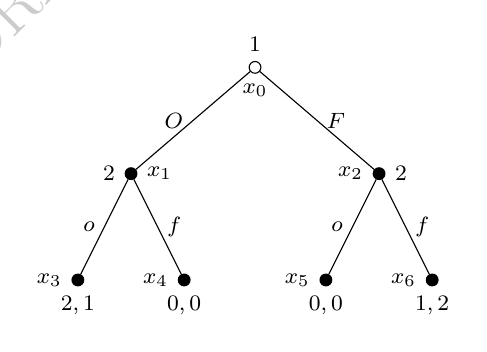
\begin{tikzpicture}[scale=0.9,font=\footnotesize,centered]
			% Specify spacing for each level of the tree
			\tikzstyle{level 1}=[level distance=15mm,sibling distance=35mm]
			\tikzstyle{level 2}=[level distance=15mm,sibling distance=15mm]	
			
			\node(0)[hollow node,label=above:{1},label=below:{$x_0$}]{}
			child{node(0-1)[solid node,label = left:{2},label = right:{$x_1$}]{} 
				child{node[solid node,label = left:{$x_3$},label = below:{$2,1$}]{} edge from parent[draw] node[left]{$o$}} 
				child{node[solid node,label = left:{$x_4$},label = below:{$0,0$}]{} edge from parent[draw] node[right]{$f$}} 
				edge from parent[draw] node[left]{$O$}}
			child{node(0-2)[solid node,label = right:{2},label = left:{$x_2$}]{} 
				child{node[solid node,label = left:{$x_5$},label = below:{$0,0$}]{} edge from parent[draw] node[left]{$o$}} 
				child{node[solid node,label = left:{$x_6$},label = below:{$1,2$}]{} edge from parent[draw] node[right]{$f$}} 
				edge from parent[draw] node[right]{$F$}}
			;
		\end{tikzpicture}
	\end{figure}
	但是上述的定义中并没有考虑每个节点上所拥有的信息,因此我们给出如下的补充
	\begin{Def}
		每个player i都有信息集合的collection \ $h_i \in H_i$,且这个collection是所有节点的partition,并且collection有如下的性质
		\begin{enumerate}
			\item 如果$h_i$是一个单元素集合,且只包含元素$x$,那么player i在x进行行动时知道他在x
			
			\item 如果$x \neq x'$且$x \in h_i,x' \in h_i$,那么在x行动的palyer不知道他在x
			
			\item 如果$x \neq x'$且$x \in h_i,x' \in h_i$,那么$A_i(x) = A_i(x')$
		\end{enumerate} 
	\end{Def}
	在博弈树上,我们可以通过连接节点来表示信息。因此在Battle of sex的博弈中可以写为
	\begin{figure}[thbp]
		\centering
		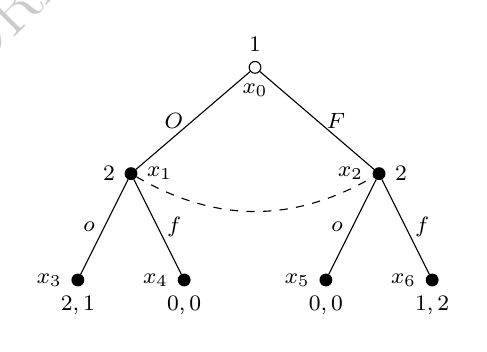
\begin{tikzpicture}[scale=0.9,font=\footnotesize,centered]
			% Specify spacing for each level of the tree
			\tikzstyle{level 1}=[level distance=15mm,sibling distance=35mm]
			\tikzstyle{level 2}=[level distance=15mm,sibling distance=15mm]	
			
			\node(0)[hollow node,label=above:{1},label=below:{$x_0$}]{}
			child{node(0-1)[solid node,label = left:{2},label = right:{$x_1$}]{} 
				child{node[solid node,label = left:{$x_3$},label = below:{$2,1$}]{} edge from parent[draw] node[left]{$o$}} 
				child{node[solid node,label = left:{$x_4$},label = below:{$0,0$}]{} edge from parent[draw] node[right]{$f$}} 
				edge from parent[draw] node[left]{$O$}}
			child{node(0-2)[solid node,label = right:{2},label = left:{$x_2$}]{} 
				child{node[solid node,label = left:{$x_5$},label = below:{$0,0$}]{} edge from parent[draw] node[left]{$o$}} 
				child{node[solid node,label = left:{$x_6$},label = below:{$1,2$}]{} edge from parent[draw] node[right]{$f$}} 
				edge from parent[draw] node[right]{$F$}}
			;
			\draw[dashed,bend right](0-1) to (0-2);
		\end{tikzpicture}
	\end{figure}
	
	在之前,我们给出了完全信息的定义,即所有player都知道其他player的行动集与payoff函数。但是对于扩展式的博弈,对于完全信息,我们还是要区分完美信息与不完美信息。
	\begin{Def}
		完全信息的博弈如果所有的信息集合都只有一个元素,且没有nature进行行动,那么就是完美信息博弈,反之就是不完美信息博弈。
	\end{Def}
	可以看到,引入nature是外生的不确定性。而信息节点有多个元素产生的不确定性是内生的不确定性。
	
	
	
	
	\subsection{策略}
	由于表达方式的不同,在动态博弈中我们需要重新定义我们的策略。我们可以首先定义以下纯策略
	\begin{Def}
		player i的纯策略是一个映射$s_i:H_i \rightarrow A_i$,对于每一个信息集合$h_i \in H_i$都分配一个动作$s_i(h_i) \in A_i(h_i)$。我们用$S_i$来表示所有的纯策略的映射。
	\end{Def}
	实际上,假设player i有$k$个信息集合,且每个信息集合有$m_i$个动作进行选择。那么纯策略就是
	\begin{equation}
		|S_i| = m_1 \times m_2 \times \cdots \times m_k
	\end{equation}
	$S_i$为$player_i$的纯策略,是$player$在所有信息集上可能的行动的笛卡尔积。
	
	接下来就是混合策略,我们可以用之前的同样方法来进行定义。纯策略是确定性的行动,混合策略则是纯策略上的概率分布。
	
	\begin{Def}
		player i的混合策略定义为在纯策略$s_i \in S_i$上的概率分布
	\end{Def}
	但是很明显,这样的定义并没有考虑到动态博弈中的动态。上述混合策略的定义中,所有的player都在博弈前直接定好了采用不同行为的概率,并不能描述$player$在一个节点上随机化自己行为的选择。以Battle of sex博弈为例,$player 2$的纯策略集合为$\{oo,,of,fo,ff\}$,上述的定义方法就不能描述“如果$player 1$选择$O$,我就选择$f$,如果$player$选择$F$,那我就以$\frac{1}{3}$的概率选择$f$”。因此我们定义一个行为策略(behavioral strategy)
	
	\begin{Def}
		一个行为策略明确了对于所有的信息集合$h_i \in H_i$,有一个在$A_i(h_i)$上的独立的概率分布,且表示为$\sigma_i:H_i \rightarrow \Delta A_i(h_i)$,且其中$\sigma_i(a_i(h_i))$代表了面对信息集合$h_i$时,player执行$a_i(h_i) \in A_i(h_i)$发生的概率。
	\end{Def}
	
	不同于混合策略,行为策略更加符合策略式博弈的动态特征。而上述的定义也可以简单的理解为,当$player$需要行动时,他会根据对应信息集上所有可能的行动来实施混合策略。
	
	现在的问题就是有这么多策略,我们是否每个种类的策略都要考虑。这就引出了行为策略和混合策略的等价性。即在特定条件下,行为策略和混合策略可以相互转换。
	
	\begin{figure}[thbp]
		\centering
		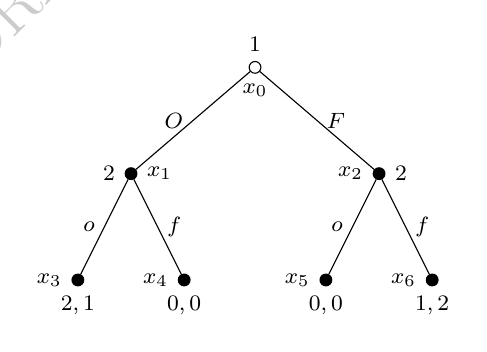
\begin{tikzpicture}[scale=0.9,font=\footnotesize,centered]
			% Specify spacing for each level of the tree
			\tikzstyle{level 1}=[level distance=15mm,sibling distance=35mm]
			\tikzstyle{level 2}=[level distance=15mm,sibling distance=15mm]	
			
			\node(0)[hollow node,label=above:{1},label=below:{$x_0$}]{}
			child{node(0-1)[solid node,label = left:{2},label = right:{$x_1$}]{} 
				child{node[solid node,label = left:{$x_3$},label = below:{$2,1$}]{} edge from parent[draw] node[left]{$o$}} 
				child{node[solid node,label = left:{$x_4$},label = below:{$0,0$}]{} edge from parent[draw] node[right]{$f$}} 
				edge from parent[draw] node[left]{$O$}}
			child{node(0-2)[solid node,label = right:{2},label = left:{$x_2$}]{} 
				child{node[solid node,label = left:{$x_5$},label = below:{$0,0$}]{} edge from parent[draw] node[left]{$o$}} 
				child{node[solid node,label = left:{$x_6$},label = below:{$1,2$}]{} edge from parent[draw] node[right]{$f$}} 
				edge from parent[draw] node[right]{$F$}}
			;
		\end{tikzpicture}
	\end{figure}
	
	还是对于Battle of sex博弈,我们考虑$player 2$的行动,他有两个节点$x_1,x_2$,因此有着两个对应的信息集$h_2^O,h_2^F$。每个信息集上他都有一个行动集$A_2 = \{o,f\}$。$player 2$的纯策略集合为$\{oo,,of,fo,ff\}$,混合策略就可以表示为$(p_{oo},p_{of},p_{fo},p_{ff})$,其中每一项都大于0,且和为1。行为策略则表示为$\sigma_2(o(h_2^O)),\sigma_2(f(h_2^O)),\sigma_2(o(h_2^F)),\sigma_2(f(h_2^F))$四个概率。且$\sigma_2(o(h_2^O)) + \sigma_2(f(h_2^O)) = 1,\sigma_2(o(h_2^F)) + \sigma_2(f(h_2^F)) = 1$
	
	为了得到等价性,我们需要考虑两个问题。一个是在给定混合策略情况下,能否用行为策略来表示。我们考虑$player 2$每个节点上的条件概率。$\Pr\{o|O\} = p_{oo} + p_{of},\Pr\{f|O\} = p_{fo} + p_{ff}$且$\Pr\{o|O\} + \Pr\{f|O\} = 1$。同样对于$player 1$的另一个策略,我们也有条件概率$\Pr\{o|F\} = p_{oo} + p_{fo},\Pr\{f|F\} = p_{of} + p_{ff}$且$\Pr\{o|F\} + \Pr\{f|F\} = 1$。因此我们可以直接得到行为策略$\sigma_2(a_2(h)) = \Pr\{a_2|h\}$
	
	另一个问题就是给定行为策略,是否可以得到混合策略。即将上述的过程反过来,求解一个线性方程组。
	
	\begin{Def}
		如果一个博弈中没有$player$会忘记他之前获得的信息,那么这个博弈就是一个\textbf{完美回忆}(perfect recall)的博弈
	\end{Def}
	
	Kuhn(1953)证明了在完美回忆博弈中,行为策略和混合策略的等价性。
	
	\subsection{NE与SPNE}
	
	extensive-form的博弈也可以表示为normal-form的博弈。而在这样的normal-form我们可以求解纳什均衡。以Battle of sex博弈为例。在静态情况下,矩阵为
	\begin{equation}
		\begin{array}{|c|c|c|}
			\hline
			1 \backslash 2 & O & F \\
			\hline
			O & 2,1 & 0,0 \\
			\hline
			F & 0,0 & 1,2 \\
			\hline
		\end{array}
	\end{equation}
	而在贯序的Battle of sex中,矩阵为
	\begin{equation}
		\begin{array}{|c|c|c|c|c|}
			\hline
			1 \backslash 2 & oo & of & fo & ff \\
			\hline
			O & 2,1 & 2,1 & 0,0 & 0,0 \\
			\hline
			F & 0,0 & 1,2 & 0,0 & 1,2 \\
			\hline
		\end{array}
	\end{equation}
	
	对于动态博弈,我们也可以用一般的方式来表示博弈。接下来我们考虑的就是如何求解出博弈中的NE。还是通过下划线法,我们就可以得到贯序的Battle of sex中的NE
	\begin{equation}
		\begin{array}{|c|c|c|c|c|}
			\hline
			1 \backslash 2 & oo & of & fo & ff \\
			\hline
			O & \underline{2},\underline{1} & \underline{2},\underline{1} & \underline{0},0 & 0,0 \\
			\hline
			F & 0,0 & 1,\underline{2} & \underline{0},0 & \underline{1},\underline{2} \\
			\hline
		\end{array}
	\end{equation}
	其中存在着三个NE,$(O,oo),(O,of),(F,ff)$。这三个NE最终展现的结果和非贯序的博弈相同,都是$(O,O),(F,F)$。实际上这里的NE和之前的定义一样,表示了一个$player$在给定其他$player$行动的信念下的最优选择。
	
	但是在动态博弈中,所有$player$的选择并不是同时决定的。因此还需要考虑选择形成的路径。
	
	\begin{Def}
		令$\sigma^* = (\sigma^*_1,\cdots,\sigma^*_n)$为extensive-form的行为策略的纳什均衡的profile。如果$\sigma^*$以正的概率到达,那么就说这个信息集合在均衡路径上。
	\end{Def}
	
	用上述的定义来说就是,在NE中,一个$player$根据他对于其他$player$在均衡路径上和均衡路径外的选择来决定选择在均衡路径上
	
	而考虑了路径后,我们上述分析的NE可能就不那么可信了。考虑$(F,ff)$,在给定$player 2$选择$ff$的正确信念下,$player 1$并不会从$F$偏离到$O$。在这里可以看作在信息集$x_1$上选择$f$是$player 2$的一种威胁。
	
	但是在信息集$x_1$上,$f$并不是一个最优的选择。因此这个威胁也就不可信了。紧接着在这种分析思路下得到的NE也并不可信。其中最主要的原因在于,在使用一般情形的表示方法中,无法显示出博弈的动态特征,所有的选择被假设为是同时进行的。
	\begin{figure}[thbp]
		\centering
		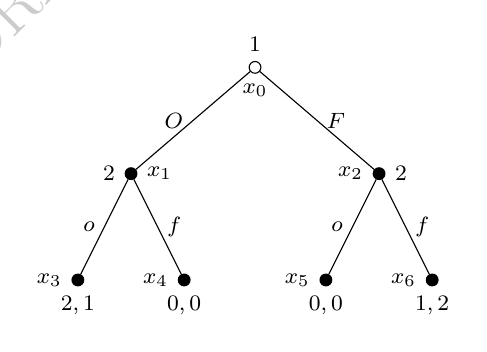
\begin{tikzpicture}[scale=0.9,font=\footnotesize,centered]
			% Specify spacing for each level of the tree
			\tikzstyle{level 1}=[level distance=15mm,sibling distance=35mm]
			\tikzstyle{level 2}=[level distance=15mm,sibling distance=15mm]	
			
			\node(0)[hollow node,label=above:{1},label=below:{$x_0$}]{}
			child{node(0-1)[solid node,label = left:{2},label = right:{$x_1$}]{} 
				child{node[solid node,label = left:{$x_3$},label = below:{$2,1$}]{} edge from parent[draw] node[left]{$o$}} 
				child{node[solid node,label = left:{$x_4$},label = below:{$0,0$}]{} edge from parent[draw] node[right]{$f$}} 
				edge from parent[draw] node[left]{$O$}}
			child{node(0-2)[solid node,label = right:{2},label = left:{$x_2$}]{} 
				child{node[solid node,label = left:{$x_5$},label = below:{$0,0$}]{} edge from parent[draw] node[left]{$o$}} 
				child{node[solid node,label = left:{$x_6$},label = below:{$1,2$}]{} edge from parent[draw] node[right]{$f$}} 
				edge from parent[draw] node[right]{$F$}}
			;
		\end{tikzpicture}
	\end{figure}
	
	然而单纯的纳什均衡可能给出一些令人困惑的解,因此我们在纳什均衡的基础上再添加\textbf{贯序理性}的假设,即player在对于在均衡路径上和路径之外会发生的情况都会进行理性的选择。定义如下
	\begin{Def}
		给定策略$\sigma_{-i} \in \Delta S_{-i}$,$\sigma_i$是贯序理性的,当且仅当$i$在他的每个信息集上都对$\sigma_{-i}$实施了最优反应。
	\end{Def}
	
	为了求解贯序理性的均衡,我们可以使用逆向归纳的方法,关于逆向归纳法,有着很有名的Zermelo's Theorem
	
	\begin{Prop}
		任何完美信息的有限博弈中,有着一个贯序理性的逆向归纳解。如果没有两个收益相同的最终节点,那么这个解是唯一的
	\end{Prop}
	
	逆向归纳法存在着局限,即只适用于完全信息的情况,因此我们还需要引入子博弈完美纳什均衡的概念。我们如下定义子博弈
	\begin{Def}
		一个extensive-form博弈$\Gamma$的真子博弈$G$包含一个节点以及这个节点后的所有节点,并且有着如下的性质。如果$x \in G,x' \in h(x)$,那么$x' \in G$。$G$本身就是一个继承了$\Gamma$的博弈树
	\end{Def}
	
	有个子博弈的概念后,我们就可以像逆向求解一样对博弈进行求解了。我们可以从最下面一层的子博弈开始求解,最后求解到根节点。这样求解的均衡也叫\textbf{子博弈完美纳什均衡},定义如下
	\begin{Def}
		令$\Gamma$为有n个player的extensive-form的博弈。当一个行为策略$\sigma^* = (\sigma^*_1,\cdots,\sigma^*_n)$对于任何一个$\Gamma$的子博弈$G$,$\sigma^*$都是$G$的一个纳什均衡时,这个策略为子博弈完美纳什均衡
	\end{Def}

	\newpage
	
	\section{多阶段博弈}
	在这里我们考虑多个不完全信息的简单博弈组合起来的博弈。即多阶段博弈。由于是不完全信息的多阶段博弈,因此在后续的阶段中,player的策略应该基于之前博弈的信息集而进行选择的。
	
	因此我们将有条件的纯策略定义为这样的形式:$S_i = \{s^1_i,s^2_i(h_1),\cdots,s^t_i(h_{t-1}),\cdots,s^T_i(h_{T-1})\}$,其中$s^t_i(h_{t-1})$表示player i在给定了信息集$h_{t-1}$的情况下,在$t$阶段做出的策略。基于这个纯策略的定义,我们也可以像之前的行为策略一样定义混合策略。
	
	对于这样的博弈,我们也想要寻找子博弈完美纳什均衡。首先我们需要定义这里的子博弈纳什均衡
	\begin{Prop}
		考虑一个$T$阶段的多阶段博弈,设$\sigma^{t*}$为第$t$阶段博弈的纳什均衡的策略profile。在多阶段博弈中存在一个子博弈完美均衡,其中均衡路径为$\sigma^{1*},\sigma^{2*},\cdots,\sigma^{T*}$
	\end{Prop}
	\begin{Prop}
		如果$\sigma^*$是包含了阶段博弈$G_1,G_2,\cdots,G_T$的多阶段博弈的纳什均衡,则$\sigma^*$在阶段$T$进行限制后的策略是那个阶段博弈的纳什均衡。
	\end{Prop}
	\begin{Prop}
		如果一个有限的多阶段博弈由各自具有唯一纳什均衡的阶段博弈组成,则该多阶段博弈具有唯一的子博弈完美均衡。
	\end{Prop}
	
	为了找到SPNE,我们使用的方法是one-stage deviation principle。很简单的想,单个stage的纳什均衡的策略结合起来是一个子博弈完美纳什均衡。但是如果在后面阶段中的博弈中存在着多个均衡,且我们可以把着两个均衡看成carrot和stick。那么我们就可能存在除了纳什均衡外的博弈。
	
	\newpage
	
	\section{重复博弈}
	
	重复博弈$G(T)$表示由相同的阶段博弈$G = \{S_1,S_2,\cdots,S_n;u_1,u_2,\cdots,u_n\}$重复$T$次。其中阶段博弈(Stage game)本身是一个完整的静态或动态博弈。与重复博弈相似的概念是序贯博弈(Sequential game)但是贯序博弈中每个阶段不是完整的博弈,即没有达到最终收益环节。
	
	经典重复博弈有着如下的特点
	\begin{enumerate}
		\item 阶段博弈间无 “物质上”的联系。即前面阶段博弈不影响后面阶段博弈的收益结构;从而参与人在各阶段博弈中无须“瞻前顾后”了解阶段收益结构。这一点对理解重复博弈解的特点和局限性很重要。
		
		\item 博弈过程有信息联系,且是共同知识。各参与人都观测到过去阶段博弈的历史。这种历史知识不影响后面阶段博弈的行动空间和收益结构(否则就不“重复”)。但可能改变后面阶段博弈中的具体选择。
	\end{enumerate}
	
	分析一个博弈,我们需要知道各个主体在博弈中得到的收益。在重复博弈中,各个参与人的总收益取决于所有阶段博弈所得收益的现值之和。
	
	因此收益与博弈重复次数$T$和贴现因子$\delta$有关。就博弈次数来说,可以分为
	\begin{enumerate}
		\item 有限重复博弈$G(T)$
		
		\item 无限重复博弈$G(\infty)$
		
		\item 随机结束的重复博弈
	\end{enumerate}
	
	贴现因子$\delta$刻画了参与者耐心程度或说时间偏好($0 \leqslant \delta \leqslant 1$),也可能源于未来能否继续博弈的不确定性。$\delta$越大,对未来越重视,越有必要跨期协调行动决策。一般假定各阶段的贴现因子不变且相等。
	
	我们来考虑一下在重复博弈中的收益。$G(T)$中的总收益为
	\begin{equation}
		u = u_1 + \delta u_2 + \delta^2 u_3 + \cdots + \delta^{T-1}u_T = \sum_{i=1}^{T}\delta^{i-1}u_i
	\end{equation}
	对应的无限重复博弈的总收益就是一个无穷级数。$G(T)$的阶段博弈平均收益,即为了得到同样的收益现值之和,在每一阶段都应得到的等额收益值 
	\begin{equation}
		\overline{u} = \frac{1-\delta}{1-\delta^T}\sum_{i=1}^{T}\delta^{i-1}u_i
	\end{equation}
	
	随机结束的重复博弈:可理解为每次阶段博弈继续的概率为$p$,结束的概率为$1-p$。(可扩展为状态依存的马尔科夫博弈)此类博弈中参与人的总收益为
	\begin{equation}
		u = (1-p)(u_1 + p \delta u_2 + p^2 \delta^2 u_3 + \cdots + p^{T-1} \delta^{T-1} u_T + \cdots) = (1-p)\sum_{i=1}^{\infty}(p \delta)^{i-1}u_i
	\end{equation}
	
	重复博弈中的策略为每个参与者的纯策略空间等于其在各个阶段博弈上策略空间的笛卡儿积。重复博弈中各阶段博弈上的策略是条件性策略,不同于单阶段博弈中的策略。
	
	我们先关注于有限重复博弈的分析。我们主要关注的是,相较于阶段博弈的均衡结果,重复博弈是否会涌现出新的均衡。
	
	基于博弈$G$中PNE个数的不同,我们有着不同的结果。
	
	\paragraph{G不存在PNE(零和博弈)的G(T)}
	
	如果$G$为零和博弈(利益严格对立竞争,你死我活,矛盾不可调和,不存在PNE),则博弈的可重复进行不会创造出新的合作激励。每个参与者在整个$G(T)$上的SPNE均衡策略,就是每次都重复单阶段博弈中的MNE策略,即以MNE所规定的概率机制选择行为。
	
	如,猜硬币博弈中,每次都各以0.5的概率正面,0.5的概率反面。这个结果之所以是SPNE,可以通过逆向推理法。因为第T阶段博弈是最后一次博弈,没有合作的机会也没有合作的必要,所以选择原零和博弈的MNE是唯一合理的选择。退回到第T-1阶段,由于预期后面不会有合作,所以本阶段也就同样不可能合作。依此类推。
	
	\paragraph{G存在唯一PNE的G(T)}
	如果该PNE对应的结果是帕累托有效的,则理性的双方为了帕累托改进,每次阶段博弈都会自动选择这一策略组合规定的策略,而重复博弈中的SPNE也就是每次都选择这一策略。如果PNE对应的结果不是帕累托有效的,结果也类似,因此有如下的一般性结论。
	
	如果阶段博弈G有唯一的NE,则任意有限重复博弈G(T),只有唯一的SPNE。该SPNE的均衡路径由各阶段博弈的NE策略组成,从而整个G(T)的SPNE结局就是单次博弈的均衡结果重复T次。即只要T有限,则重复本身不改变原阶段博弈的均衡结果,真正可谓“重复”博弈。
	
	其它非均衡路径上的各策略,尽管可能也存在着NE策略(比如连锁店悖论中进入者每次选择不进入,在位者每次选择斗争),但都不构成SPNE策略。
	
	\paragraph{G有多个NE的G(T)}
	G有多个NE时,G(T)的SPNE结果可能有多条SPNE路径,其中可能包含前面阶段有合作结果的稳
	定路径,从而合作可能内生出来。因为在多个NE下,参与人的行为可以胡萝卜与大棒并用:交替使用或触发对方使用不同的NE策略,来惩罚前面阶段的不合作行为,或奖励前面阶段的合作行为。
	
	以下图表示的博弈为例。
	\begin{equation}
		\begin{array}{|c|c|c|c|}
			\hline
			1 \backslash 2 & L & M & R \\
			\hline
			U & 0,0 & 3,4 & 6,0 \\
			\hline
			M & 4,3 & 0,0 & 0,0 \\
			\hline
			D & 0,6 & 0,0 & 5,5 \\
			\hline
		\end{array}
	\end{equation}
	
	上述博弈有两个PNE,(M,L),(U,M)和一个期望收益为(12/7,12/7)的MNE[(3/7,4/7,0),(3/7,4/7,0)]。在上述博弈中,帕累托改进的(D,R)无法在单阶段的博弈中实现,但如果重复两次,只要双方贴现因子足够大,则通过恰当的策略,可以使帕累托改进作为SPNE结局部分实现。
	
	若双方贴现因子>7/9,则如下策略具有SPNE性:第1阶段,各自分别选择(D,R)(即选择合作,传递实现帕雷托改进的愿望)。若第1阶段实现了合作,则第2阶段选择收益更高的均衡(M,L),(U,M);若第1个阶段未实现合作,则第2阶段选择MNE(收益更低的均衡,以示惩罚)。
	
	第二个阶段上,无论选择收益更高的均衡还是MNE,都是NE。因此我们主要考虑上述策略在整个$G(2)$上是否为NE。
	
	给定2遵守该策略:若1不遵守,最佳的也就是在阶段1机会主义地选U,虽多得1,但导致第2阶段损失$4-12/7$,如果$1<\delta(4-12/7)$($\delta>7/9$使这一不等式成立),则1没有动力不遵守这一合作策略;
	
	给定1遵守该策略:若2不遵守,则选择L虽多得1,但导致第2个阶段损失$3-12/7$,如果$1<\delta(3-12/7)$($\delta>7/9$使这一不等式成立), 则表明2也没有动力不遵守这一合作策略。
	
	故双方都不愿单方面不合作,因此,这一策略组合也是整个$G(2)$的一个NE,从而是一个SPNE.
	
	类似,如果重复T次,则前T-1次都选择合作,最后一次选择单阶段的另外某个
	NE策略,都是SPNE。这将实现帕雷托改进,T越大,平均收益就越接近帕雷托有效收益(5,5)。
	
	\subsection{触发策略}
	这种首先都合作,一旦发现不合作则展开
	报复性惩罚的策略,称为触发策略(trigger
	strategy)或冷酷策略(Grim strategy ).
	
	触发策略根据冷酷程度可以分为
	\begin{enumerate}
		\item 严厉触发:先合作。如果对方也一直合作,则自己继续合作。如果在某个阶段对方不合作,则自己此后都不合作。“严厉”在于一旦对方偏离合作,则触发“惩罚”,且坚持冷酷到底。
		
		\item 宽容触发:一旦触发惩罚,不是冷酷到底,而是只惩罚k个阶段,此后,重新开始传递合作愿望或者单次处罚力度降低些。“宽容”在于给对方改错的机会(给对方机会实际上也是给自己机会)
	\end{enumerate}

	触发策略是重复博弈形成合作的关键。但不一定总能内生出SPNE合作:有些博弈无法构造触发策略:因为均衡报复策略是用收益更低的均衡策略,如果只有一个NE,就无法构造这种均衡报复策略。
	
	有些触发策略不可置信:当启动报复时,也会降低自己收益。故坚持惩罚不一定是均衡策略,从而对方不一定相信。可置信性的影响因素:严厉或宽容的程度,耐心程度等。
	
	有限次重复的囚徒类博弈不必然内生出合作结果,与现实不完全相符。有两种可能打破上述困境,使陷入困境的“囚徒”实现救赎的基本途径:一是引入信息不完美来解释,见第4讲。二是使博弈重复无限次(或结束期不确定)。
	
	无限重复博弈下:如果阶段博弈G只有唯一的NE,也可能实现SPNE结果的合作:路径上每一个阶段的行动组合甚至可能不是阶段博弈的NE行动。如果阶段博弈有多个NE,则SPNE结果就更多,其中总存在一些实现帕雷托改进的。
	
	无名氏定理(Folk Theorem):无限次重复博弈(或p足够大的随机结束重复博弈)中,如果参与人对未来足够重视($\delta$足够大),那么,任何程度的合作(从而实现对单阶段NE结果的不同程度帕累托改进)都可通过某种特定的SPNE得到。

	定理意义:指出可通过设计某种重复博弈机制,实现或逼近作为SPNE合作结果的平均收益。(设计重复次数、触发策略等)
	
	\newpage
	
	\part{不完全信息静态博弈}
	
	\section{贝叶斯博弈}
	
	这章我们开始考虑不完全信息的博弈。首先信息不完全可以分为两种情况:信息不完备;信息不对称。信息不完备中某些信息对于所有的参与者而言都是不确定的。信息不对称中有一部分信息是私人信息,而非公共信息。
	
	而信息不对称也存在着两种情况
	\begin{enumerate}
		\item 关于知识信息的隐藏。参与者有意或无意地将自己的某些特征或收益信息隐藏起来,其他参与人不知道,从而这些信息成了自己的私人信息——类型t (type) 
		
		\item 关于行动信息的隐藏。参与者有意或无意地将自己的某些行动隐藏起来,没有让其他参与者知悉或观察到(主动隐藏或被动隐藏)
	\end{enumerate}
	
	
	这里的不完全信息指的是在博弈中,player并没有对于其他player的特征信息。因此在这里,player的行动就要依靠与自身对于其他player特征信息的belief。而这个belief和之前我们提到的对于action的belief有着相似之处。Harsanyi发现了这个相似之处,并构架了一个分析不完全信息的一般框架。
	
	Harsanyi最核心的分析就是,在common prior assumption假设下,所有player都知道不同player类型的分布信息,因此我们可以引入一个nature来将不完全信息转换成不完美信息(即将不同player的类型转换为nature的一种选择行为),从而使用我们之前的分析工具进行分析。
	
	在这里,我们对于不完全信息进行形式化的定义。
	\begin{Def}
		一个normal-form的n-player的不完全信息的静态博弈为
		\begin{equation}
			<N,\{A_i\}_{i=1}^n,\{\Theta_i\}_{i=1}^n,\{v_i(\cdot;\theta_i),\theta_i \in \Theta_i\}_{i=1}^n,\{\phi_i\}_{i=1}^n>
		\end{equation}
	\end{Def}
	其中$N$代表了player;$A_i$代表了i的行动集;$\Theta_i = \{\theta_{i1},\theta_{i2},\cdots,\theta_{ik_i}\}$是i的类型空间;$v_i:A \times \Theta_i \rightarrow \mathbb{R}$是i的类型依存的payoff函数;$\phi_i$表示了在明确自己的类型后,对于其他主体类型的信念。	
	
	在这里,payoff仅取决于player自身的类型,因此这是private value的类型。如果payoff取决于所有player的类型,那么这个就是common value的类型。
	
	对于一个静态的贝叶斯博弈,我们可以看作有以下几步组成
	\begin{enumerate}
		\item Nature选择一个类型的profile$(\theta_1,\theta_2,\cdots,\theta_n)$
		
		\item 每个主体i知道自己的类型$\theta_1$,然后根据$\phi_i$形成对于其他主体类型的信念
		
		\item 主体同时选择行动$a_i \in A_i,i \in N$
		
		\item 给定所有主体的行动$a = (a_1,a_2,\cdots,a_n)$,每个主体得到payoff$v_i(a;\theta_i)$
	\end{enumerate}
	
	基于这样的博弈,我们就可以定义策略
	\begin{Def}
		player i的纯策略可以表示为一个函数$s_i:\Theta_i \rightarrow A_i$,确定了当他的类型为$\theta_i$时,他选择的行动$s_i(\theta_i)$。混合策略就是在纯策略上的概率分布。
	\end{Def}
	
	给定了策略后,我们就可以定义均衡
	\begin{Def}
		一个策略的profile$s^* = (s^*_1(\cdot),s^*_2(\cdot),\cdots,s^*_n(\cdot))$是纯策略的贝叶斯-纳什均衡,当对于所有的player i,对于每个$\theta_i \in \Theta_i$,对于每个$a_i \in A_i$都有
		\begin{equation}
			\sum_{\theta_{-i} \in \Theta_{-i}}\phi_i(\theta_{-i}|\theta_i)v_i(s^*_i(\theta_i),s^*_{-i}(\theta_{-i});\theta_i)
			\geqslant
			\sum_{\theta_{-i} \in \Theta_{-i}}\phi_i(\theta_{-i}|\theta_i)v_i(a_i,s^*_{-i}(\theta_{-i});\theta_i)
		\end{equation}
		这意味着,不管player是哪个类型,他都不会改变自己的策略。
	\end{Def}
	
	不完全信息最容易导致的现象就是逆向选择,这和common value有关。
	
	\subsection{例子}
	在这里我们考虑一个例子:懦夫博弈(game of chicken)。有两个青年1和2借了父母的车来进行懦夫博弈。两个人对向驾驶,当车即将相撞时,他们有两个选择:将车向右转或者继续向前开。
	
	这里可能出现三种情况,第一种情况下,两个人都向右转,因此他们都没有任何收益,也没有任何损失;第二种情况下,一个人向右转,另一个向前开,则向前开的人赢得了所有的respect,向右转的人既没有损失,也没有收益;第三种情况下,两个人都向前开,因此两个人平分了所有的respect,但是车辆会损坏,因此他们也需要承担车辆的损失。
	
	而这些损失则取决于他们父母的类型。他们父母可能是严厉的也可能是温和的。且严厉的父母让他们承担的损失要大于温和的父母。
	
	这个博弈的策略性表示如下图所示。其中类型变量有两个,因此可能有四种不同的状态$\theta_1\theta_2 \in \{LL,LH,HL,HH\}$。而且不同的主体有着不同的信息集,对于1来说$LL,LH$在一个信息集,即他知道自己的类型为$L$,但是不知道2的类型。其他情况类似。而动作集则为$A_1 = \{C,D\},A_2 = \{c,d\}$。
	
	\begin{figure}[thbp]
		\centering
		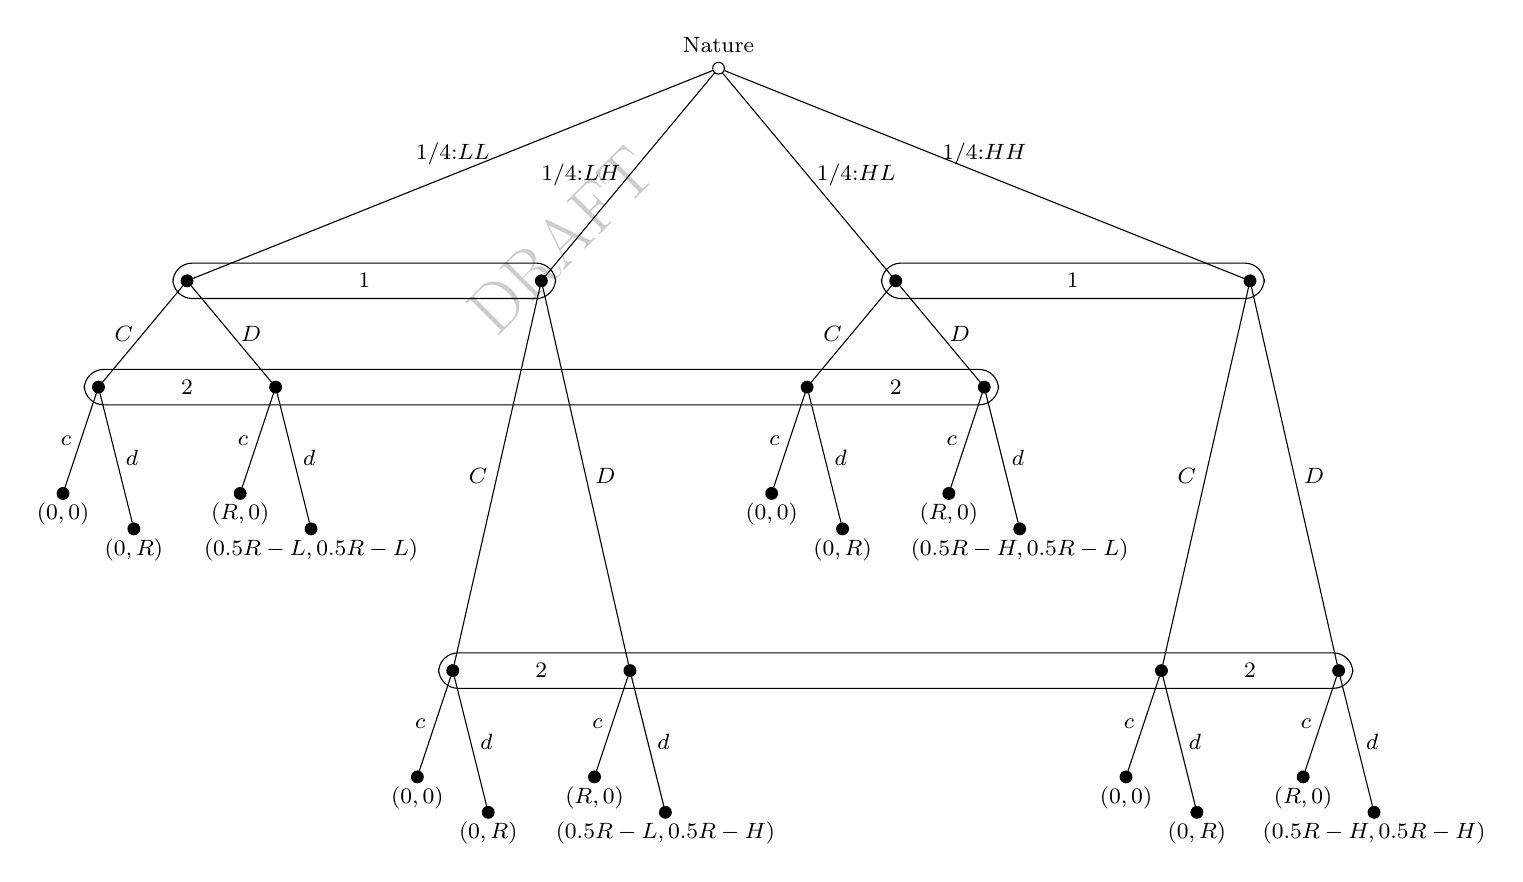
\begin{tikzpicture}[scale=0.9,font=\footnotesize,centered]
			% macro for inputing payoff vectors
			\newcommand{\payoff}[3][below]{\node[#1]at(#2){#3};}
			\newcommand{\assnum}[3][left]{\node[#1]at(#2){$x_#3$};}
			% Specify spacing for each level of the tree
			\tikzstyle{level 1}=[level distance=30mm,sibling distance=50mm]
			% \tikzstyle{level 2}=[level distance=15mm,sibling distance=30mm]	
			% \tikzstyle{level 3}=[level distance=15mm,sibling distance=30mm]	
			
			\node(0)[hollow node,label = above:{Nature}]{}
			child{
				node(0-1)[solid node]{}
				child[level distance=15mm,sibling distance=25mm]{
					node(0-1-1)[solid node]{}
					child[sibling distance=10mm]{
						node(0-1-1-1)[solid node]{}
						edge from parent[draw] node[left]{$c$}
					}
					child[level distance = 20mm,sibling distance=10mm]{
						node(0-1-1-2)[solid node]{}
						edge from parent[draw] node[right]{$d$}
					}
					edge from parent[draw] node[left]{$C$}
				}
				child[level distance=15mm,sibling distance=25mm]{
					node(0-1-2)[solid node]{}
					child[sibling distance=10mm]{
						node(0-1-2-1)[solid node]{}
						edge from parent[draw] node[left]{$c$}
					}
					child[level distance = 20mm,sibling distance=10mm]{
						node(0-1-2-2)[solid node]{}
						edge from parent[draw] node[right]{$d$}
					}
					edge from parent[draw] node[right]{$D$}
				}
				edge from parent[draw] node[above]{1/4:$LL$}
			}
			child{
				node(0-2)[solid node]{}
				child[level distance=55mm,sibling distance=25mm]{
					node(0-2-1)[solid node]{}
					child[level distance = 15mm,sibling distance=10mm]{
						node(0-2-1-1)[solid node]{}
						edge from parent[draw] node[left]{$c$}
					}
					child[level distance = 20mm,sibling distance=10mm]{
						node(0-2-1-2)[solid node]{}
						edge from parent[draw] node[right]{$d$}
					}
					edge from parent[draw] node[left]{$C$}
				}
				child[level distance=55mm,sibling distance=25mm]{
					node(0-2-2)[solid node]{}
					child[level distance = 15mm,sibling distance=10mm]{
						node(0-2-2-1)[solid node]{}
						edge from parent[draw] node[left]{$c$}
					}
					child[level distance = 20mm,sibling distance=10mm]{
						node(0-2-2-2)[solid node]{}
						edge from parent[draw] node[right]{$d$}
					}
					edge from parent[draw] node[right]{$D$}
				}
				edge from parent[draw] node[left]{1/4:$LH$}
			}
			child{
				node(0-3)[solid node]{}
				child[level distance=15mm,sibling distance=25mm]{
					node(0-3-1)[solid node]{}
					child[sibling distance=10mm]{
						node(0-3-1-1)[solid node]{}
						edge from parent[draw] node[left]{$c$}
					}
					child[level distance = 20mm,sibling distance=10mm]{
						node(0-3-1-2)[solid node]{}
						edge from parent[draw] node[right]{$d$}
					}
					edge from parent[draw] node[left]{$C$}
				}
				child[level distance=15mm,sibling distance=25mm]{
					node(0-3-2)[solid node]{}
					child[sibling distance=10mm]{
						node(0-3-2-1)[solid node]{}
						edge from parent[draw] node[left]{$c$}
					}
					child[level distance = 20mm,sibling distance=10mm]{
						node(0-3-2-2)[solid node]{}
						edge from parent[draw] node[right]{$d$}
					}
					edge from parent[draw] node[right]{$D$}
				}
				edge from parent[draw] node[right]{1/4:$HL$}
			}
			child{
				node(0-4)[solid node]{}
				child[level distance=55mm,sibling distance=25mm]{
					node(0-4-1)[solid node]{}
					child[level distance = 15mm,sibling distance=10mm]{
						node(0-4-1-1)[solid node]{}
						edge from parent[draw] node[left]{$c$}
					}
					child[level distance = 20mm,sibling distance=10mm]{
						node(0-4-1-2)[solid node]{}
						edge from parent[draw] node[right]{$d$}
					}
					edge from parent[draw] node[left]{$C$}
				}
				child[level distance=55mm,sibling distance=25mm]{
					node(0-4-2)[solid node]{}
					child[level distance = 15mm,sibling distance=10mm]{
						node(0-4-2-1)[solid node]{}
						edge from parent[draw] node[left]{$c$}
					}
					child[level distance = 20mm,sibling distance=10mm]{
						node(0-4-2-2)[solid node]{}
						edge from parent[draw] node[right]{$d$}
					}
					edge from parent[draw] node[right]{$D$}
				}
				edge from parent[draw] node[above]{1/4:$HH$}
			}
			;
			\payoff{0-1-1-1}{$(0,0)$}
			\payoff{0-1-1-2}{$(0,R)$}
			\payoff{0-1-2-1}{$(R,0)$}
			\payoff{0-1-2-2}{$(0.5R-L,0.5R-L)$}
			\payoff{0-2-1-1}{$(0,0)$}
			\payoff{0-2-1-2}{$(0,R)$}
			\payoff{0-2-2-1}{$(R,0)$}
			\payoff{0-2-2-2}{$(0.5R-L,0.5R-H)$}
			\payoff{0-3-1-1}{$(0,0)$}
			\payoff{0-3-1-2}{$(0,R)$}
			\payoff{0-3-2-1}{$(R,0)$}
			\payoff{0-3-2-2}{$(0.5R-H,0.5R-L)$}
			\payoff{0-4-1-1}{$(0,0)$}
			\payoff{0-4-1-2}{$(0,R)$}
			\payoff{0-4-2-1}{$(R,0)$}
			\payoff{0-4-2-2}{$(0.5R-H,0.5R-H)$}
			
			% information set
			\draw[rounded corners=7]($(0-1)+(-.2,.25)$)rectangle($(0-2)+(.2,-.25)$);
			\node at($(0-1)!.5!(0-2)$){1};
			
			\draw[rounded corners=7]($(0-3)+(-.2,.25)$)rectangle($(0-4)+(.2,-.25)$);
			\node at($(0-3)!.5!(0-4)$){1};
			
			\draw[rounded corners=7]($(0-1-1)+(-.2,.25)$)rectangle($(0-3-2)+(.2,-.25)$);
			\node at($(0-1-1)!.5!(0-1-2)$){2};
			\node at($(0-3-1)!.5!(0-3-2)$){2};
			
			\draw[rounded corners=7]($(0-2-1)+(-.2,.25)$)rectangle($(0-4-2)+(.2,-.25)$);
			\node at($(0-2-1)!.5!(0-2-2)$){2};
			\node at($(0-4-1)!.5!(0-4-2)$){2};
		\end{tikzpicture}
	\end{figure}
	
	从而我们可以得到每个主体的策略。1的策略为$xy \in S_1 = \{CC,CD,DC,DD\}$,其中$x$表示1为$L$时的选择,$y$表示1为$H$时的选择。同样的2也有策略$S_2 = \{cc,cd,dc,dd\}$。这里我们用策略构建矩阵来分析均衡。
	
	我们考虑一个情况下两个主体的payoff,即1选择$CD$,2选择$dd$的情况。我们可以得到1和2的期望payoff
	\begin{equation}
		\begin{aligned}
			Ev_1(CD,dd) &= \frac{1}{4} \times v_1(C,d;L) + \frac{1}{4} \times v_1(C,d;L) + \frac{1}{4} \times v_1(D,d;H) + \frac{1}{4} \times v_1(D,d;H) \\
			&= \frac{1}{4} \times 0 + \frac{1}{4} \times 0 + \frac{1}{4} \times (\frac{R}{2} - H) + \frac{1}{4} \times (\frac{R}{2} - H) = \frac{R}{4} - \frac{H}{2}
		\end{aligned}
	\end{equation}
	\begin{equation}
		\begin{aligned}
			Ev_2(CD,dd) &= \frac{1}{4} \times v_2(C,d;L) + \frac{1}{4} \times v_2(C,d;H) + \frac{1}{4} \times v_2(D,d;L) + \frac{1}{4} \times v_2(D,d;H)  \\
			&= \frac{1}{4} \times R + \frac{1}{4} \times R + \frac{1}{4} \times (\frac{R}{2} - L) + \frac{1}{4} \times (\frac{R}{2} - H) = \frac{3R}{4} - \frac{L}{4} - \frac{H}{4}
		\end{aligned}
	\end{equation}
	这里$v_i(a,b;c)$表示了在$i$为$c$类型的情况下,$i$选择$a$,其他主体选择$b$所得到的payoff。

	设$R=8,H=16,L=0$我们就可以得到如下矩阵
	\begin{equation}
		\begin{array}{|c|c|c|c|c|c|}
			\hline
			1 \backslash 2 & cc & cd & dc & dd \\
			\hline
			CC & 0,0 & 0,4 & 0,4 & \overline{0,8}\\
			\hline
			CD & 4,0 & -1,-1 & \overline{-1,3} & -6,2 \\
			\hline
			DC & 4,0 & \underline{3,-1} & \underline{\overline{3,3}} & 2,2 \\
			\hline
			DD & \underline{8,0} & 2,-6 & \overline{2,2} & -4,-4\\
			\hline
		\end{array}
	\end{equation}

	\subsection{纯化理论}
	让我们回想一下在静态博弈中出现的混合策略,考虑如下的博弈
	\begin{equation}
		\begin{array}{|c|c|c|}
			\hline
			1 \backslash 2 & H & T \\
			\hline
			H & 1,-1 & -1,1 \\
			\hline
			T & -1,1 & 1,-1 \\
			\hline
		\end{array}
	\end{equation}
	在这里,两个player的NE策略都是以$1/2$的概率来选择两个策略,因为这两个策略是无差异的。但是既然两个策略是无差异的,为什么我们需要在这两个策略之间进行随机化呢?
	
	Harsanyi提供了一个解释,并使得混合策略更加合理。首先假设两个player都对于Head有更加微小的偏好。这样payoff矩阵就如下所示。
	\begin{equation}
		\begin{array}{|c|c|c|}
			\hline
			1 \backslash 2 & H & T \\
			\hline
			H & 1 + \varepsilon_1,-1 + \varepsilon_2 & -1 + \varepsilon_1,1 \\
			\hline
			T & -1,1 + \varepsilon_2 & 1,-1 \\
			\hline
		\end{array}
	\end{equation}
	假设$\varepsilon_1,\varepsilon_2$相互独立,服从$[-\varepsilon,\varepsilon]$的均匀分布。
	
	由于分布是共同知识,但是具体的值是私人知识,因此我们可以把$\varepsilon_1,\varepsilon_2$看作是不同player的类型,从而作为一个贝叶斯博弈来进行求解。
	
	因此,整个博弈的一个类型依存的纯策略BNE可这样描述:对公司1,当$\varepsilon_1>x$时,投资;否则就不投资;对公司2,当$\varepsilon_2>y$时;投资,否则就不投资。其中,$x,y \in [-\varepsilon,\varepsilon]$。因此求解这个博弈的方法就是求出其中的$x,y$
	
	1选择H的期望收益为
	\begin{equation}
		\begin{aligned}
			&(1 + \varepsilon_1)\Pr\{\varepsilon_2 > y\} + (-1 + \varepsilon_1)\Pr\{\varepsilon_2 \leqslant y\} \\
			=&(1 + \varepsilon_1)\frac{\varepsilon-y}{2\varepsilon} + (-1 + \varepsilon_1)\frac{\varepsilon+y}{2\varepsilon} = \varepsilon_1 - \frac{y}{\varepsilon}
		\end{aligned}
	\end{equation}

	1选择T的期望收益为
	\begin{equation}
		\begin{aligned}
			&-1 \times \Pr\{\varepsilon_2 > y\} + 1 \times \Pr\{\varepsilon_2 \leqslant y\} \\
			=&-1 \times \frac{\varepsilon-y}{2\varepsilon} + 1 \times \frac{\varepsilon+y}{2\varepsilon} = \frac{y}{\varepsilon}
		\end{aligned}
	\end{equation}

	因此当$\varepsilon_1 - y/\varepsilon > y/\varepsilon$时,1选择H而不是T。即$\varepsilon_1 > 2y/\varepsilon = x$.
	
	2选择H的期望收益为
	\begin{equation}
		\begin{aligned}
			&(-1 + \varepsilon_2)\Pr\{\varepsilon_1 > x\} + (1 + \varepsilon_2)\Pr\{\varepsilon_1 \leqslant x\} \\
			=&(-1 + \varepsilon_2)\frac{\varepsilon - x}{2\varepsilon} + (1 + \varepsilon_2)\frac{\varepsilon + x}{2\varepsilon} = \varepsilon_2 - \frac{x}{\varepsilon}
		\end{aligned}
	\end{equation}

	2选择T的期望收益为
	\begin{equation}
		\begin{aligned}
			&-1 \times \Pr\{\varepsilon_1 > x\} + 1 \times \Pr\{\varepsilon_1 \leqslant x\} \\
			=&-1 \times \frac{\varepsilon-x}{2\varepsilon} + 1 \times \frac{\varepsilon+x}{2\varepsilon} = \frac{x}{\varepsilon}
		\end{aligned}
	\end{equation}
	
	因此当$\varepsilon_2 - x/\varepsilon > x/\varepsilon$时,2选择H而不是T,即$\varepsilon_2 > 2x/\varepsilon = y$
	
	联立$2x/\varepsilon = y,2y/\varepsilon = x$我们就可以得到$x= y = 0$。于是我们就得到纯策略的BNE。对于1来说,当$\varepsilon_1 > 0$时选择H,反之选择T。对于2类似。
	
	而上述纯策略在对方看来就如同以$1/2$概率进行投资的混合策略。这就是对于静态博弈的另一种诠释,也叫做纯化理论。
	
	purification theorem(海萨尼,1973):一个博弈的MNE,是某种给定的“细微扰动”(收益上的扰动)的近似博弈的纯策略BNE当扰动变量趋于无限小时的极限。
	
	混合策略的根本特征不是博弈方以随机方式选择策略,而是由于某些收益方面的不确定性造成的,当这种不确定性逐渐缩小以至消失时,在对方开来,该纯策略BNE就以极限方式退化为一个MNE。
	
	而正是自然,通过制造某种扰动,使得出现了作为不完全信息的不确定性,从而使对手感觉似乎在和选择混合策略的对手博弈。

	\newpage
	
	\section{拍卖}
	在这里,我们用贝叶斯博弈来分析拍卖。一般来说,拍卖可以分为两种,一种是open auction,其中包括了英式拍卖(The English Auction)和荷兰式拍卖(The Dutch Auction)。在open auction中,所有的拍卖者都可以看到价格动态的变化。
	
	另一种类型为sealed-bid auction,其中包括了The First-Price Sealed-Bid Auction,The Second-Price Sealed-Bid Auction。在这类型的拍卖中,所有的拍卖者同时报出自己的价格。
	
	就拍卖的分析来说,我们还可以考虑private value和common value。在private value中,拍卖者不知道其他的参与人具体的对于物品价值的判断,但是他知道分布函数。我们假设物品对player i的价值为他的类型$\theta_i \in [\underline{\theta}_i,\overline{\theta}_i]$,且服从分布函数$F(\cdot)$。如果所有的随机变量独立,那么这个情形就叫independent private values,IPV。我们首先从这个情况开始分析。
	
	在IPV的情况下,英式拍卖和The Second-Price Sealed-Bid Auction有着相同的均衡,每个参与者都会出家自己的价值。在荷兰式拍卖和The First-Price Sealed-Bid Auction也有着相同的均衡,这里的参与者都面临着增加自己的收益和增加拍卖失败的风险之间的权衡取舍。
	
	显然不同的拍卖类型之间存在着关系。我们可以用revenue equivalence theorem来进行分析。
	
	除了IPV的情况,我们还可以考虑common value的情况,这意味着一个参与者的payoff会取决于其他参与者的私有信息。这种情况下通常会导致胜者诅咒(winner's curse)
	
	\newpage
	\part{不完全信息动态博弈}
	
	\section{非完美信息下的贯序理性}
	在这章开始,我们考虑不完全信息的动态博弈。由于博弈有了动态的特征,因此我们需要新的solution concept来求解博弈。不过首先的问题是,我们是否能用之前在动态博弈中SPNE来求解博弈?
	
	考虑一个进入博弈。其中有着进入者和在位者。进入者有着两种类型,竞争性的(C)和弱的(W)。进入者首先选择是进入市场(E)还是不进入市场(O)。当进入者进入市场后,在位者可以选择跟他竞争(F)或者接受他的进入(A)。博弈的策略式表示如下
	
	\begin{figure}[thbp]
		\centering
		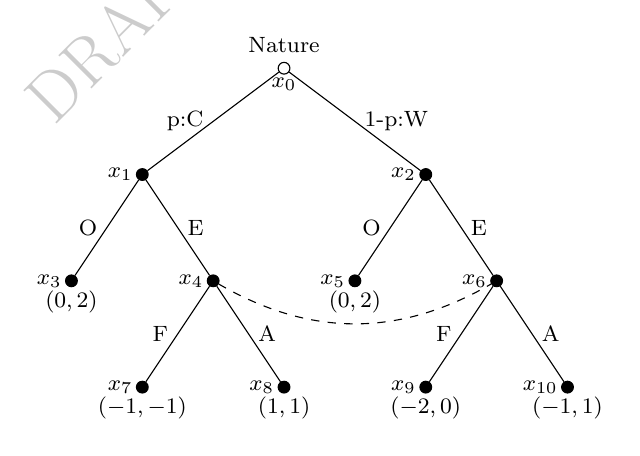
\begin{tikzpicture}[scale=0.9,font=\footnotesize,centered]
			% macro for inputing payoff vectors
			\newcommand{\payoff}[3][below]{\node[#1]at(#2){#3};}
			\newcommand{\assnum}[3][left]{\node[#1]at(#2){#3};}
			% Specify spacing for each level of the tree
			\tikzstyle{level 1}=[level distance=15mm,sibling distance=40mm]
			\tikzstyle{level 2}=[level distance=15mm,sibling distance=20mm]	
			\tikzstyle{level 3}=[level distance=15mm,sibling distance=20mm]	
			
			\node(0)[hollow node,label = above:{Nature}]{}
			child{
				node(0-1)[solid node]{}
				child{
					node(0-1-1)[solid node]{}
					edge from parent[draw] node[left]{O}
				}
				child{
					node(0-1-2)[solid node]{}
					child{
						node(0-1-2-1)[solid node]{}
						edge from parent[draw] node[left]{F}
					}
					child{
						node(0-1-2-2)[solid node]{}
						edge from parent[draw] node[right]{A}
					}
					edge from parent[draw] node[right]{E}
				}
				edge from parent[draw] node[left]{p:C}
			}
			child{
				node(0-2)[solid node]{}
				child{
					node(0-2-1)[solid node]{}
					edge from parent[draw] node[left]{O}
				}
				child{
					node(0-2-2)[solid node]{}
					child{
						node(0-2-2-1)[solid node]{}
						edge from parent[draw] node[left]{F}
					}
					child{
						node(0-2-2-2)[solid node]{}
						edge from parent[draw] node[right]{A}
					}
					edge from parent[draw] node[right]{E}
				}
				edge from parent[draw] node[right]{1-p:W}
			}
			;
			
			\assnum[below]{0}{$x_0$}
			\assnum{0-1}{$x_1$}
			\assnum{0-2}{$x_2$}
			\assnum{0-1-1}{$x_3$}
			\assnum{0-1-2}{$x_4$}
			\assnum{0-2-1}{$x_5$}
			\assnum{0-2-2}{$x_6$}
			\assnum{0-1-2-1}{$x_7$}
			\assnum{0-1-2-2}{$x_8$}
			\assnum{0-2-2-1}{$x_9$}
			\assnum{0-2-2-2}{$x_{10}$}
			
			\payoff{0-1-1}{$(0,2)$}
			\payoff{0-2-1}{$(0,2)$}
			\payoff{0-1-2-1}{$(-1,-1)$}
			\payoff{0-1-2-2}{$(1,1)$}
			\payoff{0-2-2-1}{$(-2,0)$}
			\payoff{0-2-2-2}{$(-1,1)$}
			
			\draw[dashed,bend right](0-1-2) to (0-2-2);
		\end{tikzpicture}
	\end{figure}

	我们用BNE的方法来分析上述博弈。对于1来说,他知道自己的类型信息,因此他的策略包含了自己在不同类型时的选择,即$s_1 \in S_1  = \{OO,OE,EO,EE\}$。而2只有两个策略$s_2 \in \{A,F\}$。因此策略的profile有8个。对于每个策略组合我们都可以计算出player的期望收益。设$p = 0.5$,我们就可以得到如下的矩阵
	\begin{equation}
		\begin{array}{|c|c|c|}
			\hline
			1 \backslash 2 & F & A \\
			\hline
			OO & \underline{0},\underline{2} & 0,\underline{2} \\
			\hline
			OE & -1,1 & -0.5,\underline{1.5} \\
			\hline
			EO & -0.5,0.5 & \underline{0.5},\underline{1.5} \\
			\hline
			EE & -1.5,-0.5 & 0,\underline{1}\\
			\hline
		\end{array}
	\end{equation}

	这里有两个BNE:$(OO,F)(EO,A)$。但是其中的$(OO,F)$有着不可置信的威胁。当2发现他在1选择了进入的信息集时,$F$是个严格劣策略,因此选择$F$进行威胁并不符合贯序理性。
	
	但是我们会发现,由于这里的不完全信息,整个博弈就是一个子博弈,因此上述的均衡结果也是符合SPNE的。在这样的情况下,我们不能用之前的SPNE的方法来进行分析,而应该采用新的solution concept。
	
	\subsection{完美贝叶斯均衡}
	接下来我们就来考虑新的solution concept。但是首先要引入之前在动态博弈中引入的在均衡路径以及不在均衡路径的定义。
	
	\begin{Def}
		令$\sigma^* = (\sigma^*_1,\cdots,\sigma^*_n)$为不完全信息博弈中BNE策略的profile。如果在给定$\sigma^*$和类型的分布下,信息集会以正的概率到达,那么这个信息集就\textbf{在均衡路径上}(on the equilibrium path)。相反如果以0概率到达,那么这个信息集就\textbf{不在均衡路径上}(off the equilibrium path)。
	\end{Def}
	
	以之前的博弈为例,当1选择$EO$策略时,他的两个信息集分别以$p,1-p$的概率达到,而2的信息集则以$p$的概率达到,因此所有的信息集都在均衡路径上。当1选择$OO$策略时,他的两个信息集仍然会以正的概率达到,而2的信息则不再均衡路径上。
	
	而之前的$(OO,F)$策略不可置信就是因为他没有考虑不在均衡路径上的信息集。
	
	此外在所有player的每个信息集上都有belief
	\begin{Def}
		一个策略式表示的博弈的system of belief \ $\mu$给每个信息集分配了一个关于决策节点的概率分布。也就是说对于每个信息集$h \in H$,每个决策节点$x \in h$,$\mu(x) \in [0,1]$是一个信息集中,player在决策节点$x$的概率,其中$\sum_{x \in h}\mu(x) = 1,\forall h \in H$
	\end{Def}
	
	上述的belief其实就是用概率将信息集内的节点进行了分解。由于在子博弈中,信息集不能分解,因此我们就用信念来进行分解。还是考虑上述的博弈,在其中1的所有信息集都是单点集,因此已经是well-defined的了。对于2来说,$x_4,x_6$在同一个信息集,因此需要定义$\mu(x_4)$来表示他在$x_4$的信念。
	
	为了给出在不完全信息下的贯序理性,我们还需要考虑贯序理性的几个要求。
	\begin{Req}
		每个player在他的信息集上都有well-defined的belief。也就是说这个博弈有system of belief
	\end{Req}

	首先第一个要求就是这个博弈需要system of belief。接下来的问题就是这个belief是如何决定的。belief受到两种约束,一种是其他player的行动,也叫做\textbf{信念的内生约束}(endogenous constraint on beliefs);另一种是Nature对于player类型的选择,也叫做\textbf{信念的外生约束}(exogenous constraint on beliefs)。
	
	以之前的例子举例,我们考虑一下$\mu(x_4)$,他表示了2对于他在信息集中为$x_4$节点的信念,即在1选择$E$的情况下,1为竞争类型的概率。同样我们也可以知道$1 - \mu(x_4)$
	\begin{equation}
		\begin{aligned}
			\mu(x_4) &= \Pr\{player \ 1 \ is \ competitive | E\} \\
			1 - \mu(x_4) &= \Pr\{player \ 1 \ is \ weak | E\}
		\end{aligned}
	\end{equation}

	给定具体例子,假设2相信1会采取策略$EO$,那么这时候$\mu(x_4) = 1$,因为首先Nature会给定p的概率选择1为competitive,此时1进入市场;Nature给定1-p的概率选择1为weak,此时1不进入市场。因此在2的信息集中,他100\%会处在$x_4$。
	
	上述简单描述了信念如何取决于外生和内生的约束,当然其中1可以选择比$EO$更加复杂的策略。例如混合策略/行为策略,考虑1的策略,当1的类型为$\theta_1 = C$是,用$\sigma_C$的概率实施$E$,$1-\sigma_C$的概率实施$O$。当类型为$\theta_1 = W$时,用$\sigma_W$的概率实施$E$,$1-\sigma_W$的概率实施$O$。因此我们可以运用贝叶斯法则
	\begin{equation}
		\begin{aligned}
			\mu(x_4)
			&= \Pr\{1 \ is \ competitive | entry \ occurred\} \\
			&= \dfrac{\Pr\{competitive \ and \ entry \ occurred\}}{\Pr\{competitive \ and \ entry \ occurred\} + \Pr\{weak \ and \ entry \ occurred\}} \\
			&= \dfrac{p\sigma_C}{p\sigma_C + (1-p)\sigma_W}
		\end{aligned}
	\end{equation}
	纯策略$EO$其实就是$\sigma_C = 1,\sigma_W = 0$。我们第二个要求考虑的就是上述所说的关于belief的约束
	\begin{Req}
		令$\sigma^* = (\sigma^*_1,\cdots,\sigma^*_n)$为BNE策略的profile。所有在均衡路径上的信息集的belief都需要与贝叶斯定律一致
	\end{Req}
	在均衡路径上的信息集有着两种约束,那么在均衡路径外的信息集有着如下的要求
	\begin{Req}
		均衡路径外的任何信息集可以被赋予任何信念
	\end{Req}
	以上我们考虑了关于信念的要求,最后我们考虑和信念有关的贯序理性的要求
	\begin{Req}
		给定信念后,每个player的策略都必须是贯序理性的,即在每个信息集,player都做出对于他信念的最优反应。
	\end{Req}
	形式化的表达就是
	\begin{equation}
		E[v_i(\sigma_i,\sigma_{-i},\theta_i)|h,\mu] \geqslant E[v_i(s'_i,\sigma_{-i},\theta_i)|h,\mu],\forall s'_i \in S_i
	\end{equation}

	根据上述的四个要求,我们就可以剔除我们之前分析中那些不可置信的均衡。
	
	根据上述四个要求我们也可以得出一个新的solution concept
	\begin{Def}
		如果一个BNE的profile$\sigma^* = (\sigma^*_1,\cdots,\sigma^*_n)$和一个system of belief$\mu$满足上述四个要求,那么他们就组成了完美贝叶斯均衡(perfect Bayesian equilibrium,PBE)
	\end{Def}
	为了找到PBE,我们首先需要找到BNE,然后在根据system of belief来验证BNE是否为PBE。根据上述的要求我们也可以很简单的得出如下命题
	\begin{Prop}
		如果一个贝叶斯博弈$\Gamma$的BNE的profile$\sigma^* = (\sigma^*_1,\cdots,\sigma^*_n)$包含的所有信息集都能以正的概率达到。那么$\sigma^*$和由$\sigma^*$以及类型的分布得到的唯一的belief system构成了一个PBE
	\end{Prop}

	由于上述的定义中,要求三并没有对于均衡路径外的信息集添加约束,因此上述的solution concept也叫做weak perfect Bayesian equilibrium。与之对应更加严格的PBE则要求均衡路径外的信息集也符合贝叶斯定律。
	
	上述就是对于PBE的再一步精炼。对于均衡路径外的信息的信念添加约束,也叫做贯序均衡。
	
	从具有私人信息的参与者的角度看,PBE有3类可能情形:
	\begin{enumerate}
		\item 分离均衡(separating Equilibrium):不同类型的参与者理性地选择不同的行动,行动传递准确的类型信息,后验信念均变成退化的。
		
		\item 混同均衡(pooling Equilibrium),不同类型的代理人都理性地选择相同的行动,行动不传递类型信息,信念得不到修正。
		
		\item 混杂均衡(Mixed Equilibrium) :部分参与人选择不同的行动,部分参与人则随机选择行动(可能相同,也可能不同),行动传递部分信息,信念也部分得到修正。
	\end{enumerate}
	
	\newpage 
	
	\section{信号博弈}
	在不完全信息中,一方的类型为私人信息,而在某些博弈中,拥有私人信息的player可能希望揭示自己的信息。以上这又有着信息传递的博弈叫做信号博弈(Signaling games),一般来说有着如下的结构
	\begin{enumerate}
		\item Nature选择1的类型,2不知道,但是收益取决于这个类型,集common values
		
		\item 1有着至少和类型一样多的行动集,且对于不同类型,每个行动的成本都不同
		
		\item 1选择一个行动,2根据1的行动回应
		
		\item 给定2关于1策略的belief,2在观察到1的行动后更新自己的belief并根据更新后的belief实施best response
	\end{enumerate}
	接下来我们具体考虑几个例子
	
	\subsection{MBA Game}
	上述博弈考虑了学位在劳动力市场中发出信号的作用。具体来说有着如下的步骤
	\begin{enumerate}
		\item Nature选择1的类型,可能时高生产力的(H),也可能是低生产力的(L),且满足common prior assumption。
		
		\item 1得知自己的类型后,选择获得一个MBA学位(D)或者保持本科(U)。不同类型获得学位需要付出不同成本$c_H,c_L$,且$c_H < c_L$,设$c_H = 2,c_L = 5$
		
		\item 2是雇佣者,可以让1成为经理(M)或者蓝领工人(B)。不同的职位有着不同的工资$w_M,w_B$,且$w_M > w_B$,设$w_M = 10,w_B = 6$
		
		\item 2的收益取决于雇佣人能力和职位的匹配程度,如下矩阵所示
		\begin{equation}
			\begin{array}{|c|c|c|}
				\hline
				 & M & B \\
				 \hline
				 H & 10 & 5 \\
				 \hline
				 L & 0 & 3 \\
				 \hline
			\end{array}
		\end{equation}
	\end{enumerate}

	整体的博弈树如下图所示,我们令第一个信息集为$I_U$,第二个信息集为$I_D$。接下来考虑1可能的策略,以及与策略相关的信念。
	\begin{figure}[thbp]
		\centering
		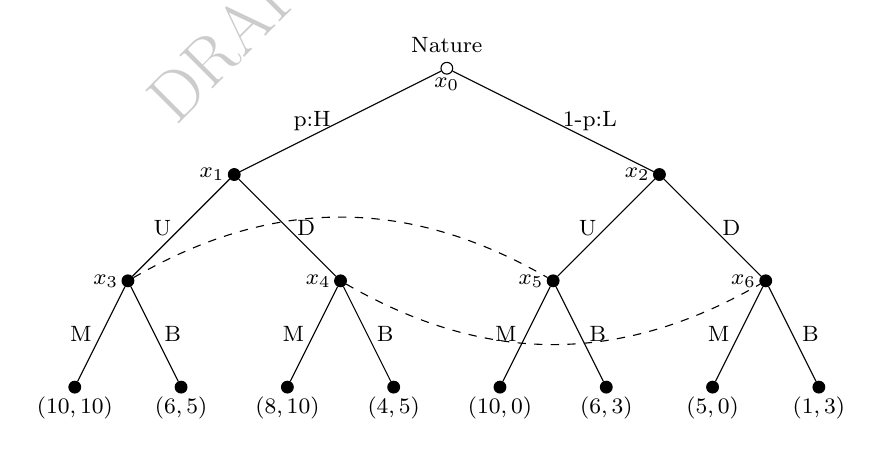
\begin{tikzpicture}[scale=0.9,font=\footnotesize,centered]
			% macro for inputing payoff vectors
			\newcommand{\payoff}[3][below]{\node[#1]at(#2){#3};}
			\newcommand{\assnum}[3][left]{\node[#1]at(#2){#3};}
			% Specify spacing for each level of the tree
			\tikzstyle{level 1}=[level distance=15mm,sibling distance=60mm]
			\tikzstyle{level 2}=[level distance=15mm,sibling distance=30mm]	
			\tikzstyle{level 3}=[level distance=15mm,sibling distance=15mm]	
			
			\node(0)[hollow node,label = above:{Nature}]{}
			child{
				node(0-1)[solid node]{}
				child{
					node(0-1-1)[solid node]{}
					child{
						node(0-1-1-1)[solid node]{}
						edge from parent[draw] node[left]{M}
					}
					child{
						node(0-1-1-2)[solid node]{}
						edge from parent[draw] node[right]{B}
					}
					edge from parent[draw] node[left]{U}
				}
				child{
					node(0-1-2)[solid node]{}
					child{
						node(0-1-2-1)[solid node]{}
						edge from parent[draw] node[left]{M}
					}
					child{
						node(0-1-2-2)[solid node]{}
						edge from parent[draw] node[right]{B}
					}
					edge from parent[draw] node[right]{D}
				}
				edge from parent[draw] node[left]{p:H}
			}
			child{
				node(0-2)[solid node]{}
				child{
					node(0-2-1)[solid node]{}
					child{
						node(0-2-1-1)[solid node]{}
						edge from parent[draw] node[left]{M}
					}
					child{
						node(0-2-1-2)[solid node]{}
						edge from parent[draw] node[right]{B}
					}
					edge from parent[draw] node[left]{U}
				}
				child{
					node(0-2-2)[solid node]{}
					child{
						node(0-2-2-1)[solid node]{}
						edge from parent[draw] node[left]{M}
					}
					child{
						node(0-2-2-2)[solid node]{}
						edge from parent[draw] node[right]{B}
					}
					edge from parent[draw] node[right]{D}
				}
				edge from parent[draw] node[right]{1-p:L}
			}
			;
			
			\assnum[below]{0}{$x_0$}
			\assnum{0-1}{$x_1$}
			\assnum{0-2}{$x_2$}
			\assnum{0-1-1}{$x_3$}
			\assnum{0-1-2}{$x_4$}
			\assnum{0-2-1}{$x_5$}
			\assnum{0-2-2}{$x_6$}
			
			
			\payoff{0-1-1-1}{$(10,10)$}
			\payoff{0-1-1-2}{$(6,5)$}
			\payoff{0-1-2-1}{$(8,10)$}
			\payoff{0-1-2-2}{$(4,5)$}
			\payoff{0-2-1-1}{$(10,0)$}
			\payoff{0-2-1-2}{$(6,3)$}
			\payoff{0-2-2-1}{$(5,0)$}
			\payoff{0-2-2-2}{$(1,3)$}
			
			\draw[dashed,bend right](0-1-2) to (0-2-2);
			\draw[dashed,bend left](0-1-1) to (0-2-1);
		\end{tikzpicture}
	\end{figure}
	
	令$\sigma^H$表示类型为$H$的1选择策略$U$的概率,$\sigma^L$表示类型为$L$的1选择策略$U$的概率。因此我们可以计算在不同决策点的信念。在信息集$I_U$中,在决策点$x_3$的信念$\mu_U$为
	\begin{equation}
		\mu_U = \dfrac{p\sigma^H}{p\sigma^H + (1-p)\sigma^L}
	\end{equation}
	在信息集$I_D$中,在决策点$x_4$的信念$\mu_D$为
	\begin{equation}
		\mu_D = \dfrac{p(1-\sigma^H)}{p(1-\sigma^H) + (1-p)(1-\sigma^L)}
	\end{equation}
	求解博弈的PBE还是一样的方法,先转换成normal-form寻找BNE,然后再根据信念验证PBE。为了求解方便,我们假设$p = 1/4$。
	
	首先考虑纯策略的情况,1的纯策略可以表示为$a_1^Ha_1^L$,即状态依存的行动。2的纯策略可以表示为$a_2^Ua_2^D$,即依赖于1的行动的行动。每个player都有四个纯策略,因此总共有16个纯策略。收益矩阵为
	\begin{equation}
		\begin{array}{|c|c|c|c|c|}
			& MM & MB & BM & BB \\
			UU & 10,2.5 & 10,2.5 & 6,3.5 & 6,3.5 \\
			UD & 6.25,2.5 & 3.25,4.75 & 5.25,1.25 & 2.25,3.5  \\
			DU & 9.5,2.5 & 8.5,1.25 & 6.5,4.75 & 4.5,3.5\\
			DD & 5.75,2.5 & 1.75,3.5 & 5.75,2.5 & 1.75,3.5 \\
		\end{array}
	\end{equation}
	
	\newpage
	
	\part{补充}
	
	\section{策略性行动}
	博弈中某些参与人所采取的一种可观察且不可逆转的行动,其目的在于:通过影响博弈中其他人对我会如何行为的预期,从而促使对方最后选择的行动,也能增进我的利益。
	
	原博弈为静态时,各方都可采取。此时将使博弈由静态变成两阶段的动态博弈。
	
	原博弈为动态时,行动顺序在后的人可能有必要采用。此时相当于增加了一个博弈阶段。
	
	策略性行为和子博弈动态精炼思想在两方面有着关系。从逻辑上讲:子博弈动态精炼是策略性行动的理论基础:策略性行动理论,只有利用子博弈动态精炼的思想,才能预先分析和发现应采用何种行动,去改变博弈的原有均衡,促成能更大限度增进自身利益的均衡结局。
	
	从起源上讲:策略性行动思想提出在先,子博弈动态精炼思想出现在后:Schelling的一系列论文先提出并运用策略性行动思想,分析现实中的各种冲突与合作应对;Selten受此启发,提出对静态NE进行子博弈精炼的思想,成为最重要的一种精炼。
	
	策略性行为按行动是否是条件依存的分为两类
	\begin{enumerate}
		\item 无条件的。这类策略行动称为Commitment(承诺),其所包含的行动内容,不依赖于对方采取什么行动这一条件。
		
		\item 条件依存的。这类行动具体内容如何触发,依赖于对方将采取的行动如何。相当于是对对方可能采取的行动实现公布了一个反应规则或者说反应函数。不过,博弈理论中,有时候这两类被混淆,用Commitment概称所有的策略性行动。
	\end{enumerate}

	条件依存型策略性行动,按对其他参与者“影响”是有利还是不利,又分为两类
	\begin{enumerate}
		\item 威胁。这类行动最终会降低其他参与人利益;使对方理性地放弃原有最优策略选择,故是“威胁”。
		
		策略中包含的行动内容,最终是否全部得以践行,前提是对方是否做出了不希望做的行为。通常威胁是\textbf{无成本}的。
		
		\item 允诺。这类行动最终也会增进其他参与人的利益(双赢)即形成利益诱导,如果对方理性地放弃原有最优策略,则该允诺的内容将生效。容易与无条件的Commitment混淆。行动方的单方行为:策略中所含行动,已直接付诸实施。通常允诺是\textbf{有成本}的。
	\end{enumerate}
	
	公开可观察的有效策略性行动,要求可置信(Credible):采取该策略性行动的参与者,必须使其他参与者知道并且相信,自己采取该行动是符合个人理性的:即比起不采取,采取时能提高收益或规避更多损失;否则,就是不可置信,从而无效。
	
	可置信的策略性行动的本质:“对于选择的自由的一种有限自愿但却又不能反悔的牺牲。”(Schelling)
	
	\begin{enumerate}
		\item 有限自愿:事前理性要求自愿:博弈前,预先采取这一策略符合个人理性:即能增进利益或规避损失。有限:牺牲自由当然不太愿意,毕竟是一种额外成本。
		
		\item 不能反悔:事后理性要求博弈过程中,若出现该策略所指向的情况,遵循这一策略符合个人理性(主动或被动)。否则就是空头威胁或空头承诺。
	\end{enumerate}

	策略性行动通常有着以下几种手段
	\begin{enumerate}
		\item 缩小行动空间。使自己的某项行动选择完全没有可能。例如破釜沉舟、背水一战。
		
		\item 改变收益结构。增加自己某项选择的成本。
		
		\item 策略运用沉没成本。使某些事后才需视情况付出的成本,在事前就支付出去,且不能收回(沉没了)。
		
		\item 建立声誉。为提高策略性行动的可置信性,声誉很重要。
	\end{enumerate}

	我们考虑一个运用策略性行为的例子-诉讼博弈(Rosenberg,1985,Rasmusen,1994)。模型意图解释一类普遍现象:为什么名人大企更易受“花边”指控;为什么他们更喜欢聘请常年律师之类,避免各种“花边”敲诈。
	
	在模型中存在两个主体原告P与被告D。原告P:指控成本$c$; “私了”要价$s$;起诉成本$p$,胜诉概率$\gamma$;胜诉所得赔偿$X$;且$c < \gamma X < p$。被告D有着应诉成本$d$,其中包含了声誉损失,且一般远大于$p$。
	
	我们考虑三种情况,首先是没有策略性行为的情况下;其次是被告和原告都采取事先雇佣常年律师的策略性行为。
	
	\begin{figure}[thbp]
		\centering
		\begin{tikzpicture}[scale=0.9,font=\footnotesize,centered]
			% macro for inputing payoff vectors
			\newcommand{\payoff}[3][below]{\node[#1]at(#2){#3};}
			% Specify spacing for each level of the tree
			\tikzstyle{level 1}=[level distance=15mm,sibling distance=30mm]
			\tikzstyle{level 2}=[level distance=15mm,sibling distance=30mm]	
			\tikzstyle{level 3}=[level distance=15mm,sibling distance=30mm]	
			
			\node(0)[hollow node,label=above:{Prosecutor},label=below:{$x_0$}]{}
			child{node(0-1)[solid node,label = left:{$x_1$}]{}
				edge from parent[draw] node[left]{不指控}
			} 
			child{node(0-2)[solid node,label = right:{Defendant},label = left:{$x_2$}]{} 
				child{
					node(0-2-1)[solid node,label = left:{Prosecutor},label = right:{$x_3$}]{} 
					child{
						node(0-2-1-1)[solid node,label = left:{$x_5$}]{}
						edge from parent[draw] node[left]{起诉}
					}
					child{
						node(0-2-1-2)[solid node,label = left:{$x_6$}]{}
						edge from parent[draw] node[right]{放弃}
					}
					edge from parent[draw] node[left]{应诉}
				} 
				child{
					node(0-2-2)[solid node,label = left:{$x_4$}]{} 
					edge from parent[draw] node[right]{接受}
				} 
				edge from parent[draw] node[right]{指控}
			}
			;
			\payoff{0-1}{$(0,0)$}
			\payoff{0-2-2}{$(s-c,-s)$}
			\payoff{0-2-1-1}{$(\gamma X - c - p,-\gamma X - d)$}
			\payoff{0-2-1-2}{$(-c,0)$}
		\end{tikzpicture}
		\caption{诉讼博弈的博弈树}
	\end{figure}

	我们可以用SPNE的方法来对上述博弈进行分析。在$x_3$点由于$\gamma X - p < 0$,因此Prosecutor会选择放弃。在$x_2$点,由于$0 > -s$,因此Defedant会选择应诉。最后在$x_0$,由于$0 > -c$,因此Prosecutor会选择不指控。因此SPNE为((不指控,放弃),应诉)。
	
	在这里,P的起诉威胁不可置信,达不到敲诈目的。因此我们接下来考虑他能否采取什么策略性行动,使起诉威胁变得可置信从而使敲诈成功获益。
	
	接下来我们考虑P的策略性行为,即支付律师费p聘请常年律师应对。则博弈树如图6.2所示
	\begin{figure}[thbp]
		\centering
		\begin{minipage}[t]{0.48\textwidth}
			\centering
			\begin{tikzpicture}[scale=0.9,font=\footnotesize,centered]
				% macro for inputing payoff vectors
				\newcommand{\payoff}[3][below]{\node[#1]at(#2){#3};}
				\newcommand{\assnum}[3][left]{\node[#1]at(#2){#3};}
				% Specify spacing for each level of the tree
				\tikzstyle{level 1}=[level distance=15mm,sibling distance=15mm]
				\tikzstyle{level 2}=[level distance=15mm,sibling distance=30mm]	
				\tikzstyle{level 3}=[level distance=15mm,sibling distance=30mm]	
				
				\node(0-0)[hollow node,label = left:{Prosecutor}]{}
				child{
					node(0)[solid node,label=left:{Prosecutor}]{}
					child{
						node(0-1)[solid node]{}
						edge from parent[draw] node[left]{不指控}
					} 
					child{
						node(0-2)[solid node,label = right:{Defendant}]{} 
						child{
							node(0-2-1)[solid node,label = left:{Prosecutor}]{} 
							child{
								node(0-2-1-1)[solid node]{}
								edge from parent[draw] node[left]{起诉}
							}
							child{
								node(0-2-1-2)[solid node]{}
								edge from parent[draw] node[right]{放弃}
							}
							edge from parent[draw] node[left]{应诉}
						} 
						child{
							node(0-2-2)[solid node]{} 
							edge from parent[draw] node[right]{接受}
						} 
						edge from parent[draw] node[right]{指控}
					}
					edge from parent[draw] node[right]{支出律师费$p$}
				}
				;
				\payoff{0-1}{$(-p,0)$}
				\payoff{0-2-2}{$(s-c-p,-s)$}
				\payoff{0-2-1-1}{$(\gamma X - c - p,-\gamma X - d)$}
				\payoff{0-2-1-2}{$(-c-p,0)$}
				
				\assnum[right]{0-0}{$x_0$}
				\assnum[right]{0}{$x_1$}
				\assnum{0-1}{$x_2$}
				\assnum{0-2}{$x_3$}
				\assnum[right]{0-2-1}{$x_4$}
				\assnum{0-2-2}{$x_5$}
				\assnum{0-2-1-1}{$x_6$}
				\assnum{0-2-1-2}{$x_7$}
			\end{tikzpicture}
			\caption{Prosecutor支出律师费的博弈树}
		\end{minipage}
		\begin{minipage}[t]{0.48\textwidth}
			\centering
			\begin{tikzpicture}[scale=0.9,font=\footnotesize,centered]
				% macro for inputing payoff vectors
				\newcommand{\payoff}[3][below]{\node[#1]at(#2){#3};}
				\newcommand{\assnum}[3][left]{\node[#1]at(#2){$x_#3$};}
				% Specify spacing for each level of the tree
				\tikzstyle{level 1}=[level distance=15mm,sibling distance=15mm]
				\tikzstyle{level 2}=[level distance=15mm,sibling distance=30mm]	
				\tikzstyle{level 3}=[level distance=15mm,sibling distance=30mm]	
				
				\node(0-0-0)[hollow node,label = left:{Defendant}]{}
				child{
					node(0-0)[hollow node,label = left:{Prosecutor}]{}
					child{
						node(0)[solid node,label=left:{Prosecutor}]{}
						child{
							node(0-1)[solid node]{}
							edge from parent[draw] node[left]{不指控}
						} 
						child{
							node(0-2)[solid node,label = right:{Defendant}]{} 
							child{
								node(0-2-1)[solid node,label = left:{Prosecutor}]{} 
								[sibling distance = 38mm]
								child{
									node(0-2-1-1)[solid node]{}
									edge from parent[draw] node[left]{起诉}
								}
								child{
									node(0-2-1-2)[solid node]{}
									edge from parent[draw] node[right]{放弃}
								}
								edge from parent[draw] node[left]{应诉}
							} 
							child{
								node(0-2-2)[solid node]{} 
								edge from parent[draw] node[right]{接受}
							} 
							edge from parent[draw] node[right]{指控}
						}
						edge from parent[draw] node[right]{支出律师费$p$}
					}
					edge from parent[draw] node[right]{支出律师费$d_1$}
				}
				
				
				;
				\payoff{0-1}{$(-p,-d_1)$}
				\payoff{0-2-2}{$(s-c-p,-s-d_1)$}
				\payoff{0-2-1-1}{$(\gamma X - c - p,-\gamma X - d_1 - d_2)$}
				\payoff{0-2-1-2}{$(-c-p,-d_1)$}
				
				\assnum[right]{0-0-0}{0}
				\assnum[right]{0-0}{1}
				\assnum[right]{0}{2}
				\assnum{0-1}{3}
				\assnum{0-2}{4}
				\assnum[right]{0-2-1}{5}
				\assnum{0-2-2}{6}
				\assnum{0-2-1-1}{7}
				\assnum{0-2-1-2}{8}
			\end{tikzpicture}
			\caption{Defendant支出律师费的博弈树}
		\end{minipage}
	\end{figure}
	
	首先考虑$x_4$,此时$\gamma X - c - p > -c -p$,因此Prosecutor会起诉。在$x_3$,由于d比较打,因此$s < \gamma X + d$,接受私了是Defendant的最优策略。在$x_1$,只要$s>c$,那么Prosecutor也会希望私了,且P不仅希望收回指控成本,还希望收回比起诉更高的收益,即$s-c-p > \gamma X - c - p$。因此P在涉及要价时会设$s > \gamma X$
	
	所以,若P将$s$定在$(\gamma X,\gamma X + d)$,对方会接受私了。此时SPNE结果变为((指控,起诉),接受)。名人由于声誉问题,d很大,故起诉成了可置信的威胁,P有很大动力去指控。这可以部分解释为什么名人或大企更容易受到“花边”指控。
	
	面对原告上述策略,被告也能采取策略性行为来应对。这里我们考虑被告之前就用小于应诉成本$d$的费用$d_1$聘请私人律师的行动。其中$d_2<d$为应诉的其他损失。此时博弈树如图6.3所示

	在$x_5$,Prosecutor的最优选择仍然是起诉。在$x_4$时,仅当$-s - d_1 > -\gamma X - d_1 - d_2$,即$s < \gamma X + d_2$时,Defendant才会选择接受。在$x_2$时,私了的前提仍然是$s > \gamma X$。
	
	作为SPNE结果,P的私了要求空间缩小为:$(\gamma X,\gamma X + d_2)$,远小于原来的私了空间。D通过提前支付律师费的策略性行动,大大降低了花边敲诈的可能性。


	
	\newpage
	
	\section{演化博弈}
	
	我们直接由例子引入。考虑一种甲虫种群,假设每只甲虫对给定环境的适应能力取决于 它是否可以发现食物,能否有效地从食物中汲取营养假设一个特定的突变基因出现并开始蔓延,造成携带该突变基因的甲虫体型变大。现在,在该甲虫种群中,便分成两种不同的群体——小甲虫和大甲虫。这两个群体最终的比率会如何呢?
	
	此时,每只甲虫有两个基因选择策略:大体态和小体态。每只甲虫从争夺一定量食物的互动中获得的生物适应性(Fittness,不一定是直接的食物量,因为不同大小消耗也不一样,同量食物可能导致的适应性不同),可认为是双主体博弈中的收益。
	
	每只甲虫的策略都由遗传基因硬性决定, “策略选择”概念在此缺失 ,以策略选择为基础的纳什均衡思想也就没有直接对应。演化博弈论首先构造了一个平行概念--“演化稳定策略”对应,作为分析稳定趋势的基础。
	
	\begin{equation}
		\begin{array}{|c|c|c|}
			\hline
			1 \backslash 2 & Small & Big \\
			\hline
			Small & 5,5 & 1,8 \\
			\hline
			Big & 8,1 & 3,3 \\
			\hline
		\end{array}
	\end{equation}
	
	演化稳定策略(ESS)定义:一个策略称为是演化稳定的,若当整个种群都采取这个策略时,任何采用不同策略的小规模 “入侵”群体经过多代遗传后最终会消亡。即该策略具有抵御小规模群体入侵或变异的能力。
	
	为了形式化描述ESS,我们首先需要描述两个概念。生物体的适应性:用它与一随机遇到的生物体互动得到的收益期望代表。
	
	称“策略T在x程度上(以x水平)入侵策略S”: 在总体中有x占比的生物体采用策略T,1-x占比采用策略S。$x \in (0,1)$
	
	ESS:若存在一个小正数y,当任何其他策略T以任何x<y水平入侵策略S时,采用策略S的个体的适应性严格高于采取策略T的个体,则称策略S是演化稳定的(evolutionarily stable)
	
	将ESS运用到上述模型中,考虑一个小正数$x$总体中有$x$占比的个体使用大体态入侵。$1-x$占比使用小体态。
	
	小甲虫的期望收益为$5 \times (1-x) + 1 \times x = 5 - 4x$;大甲虫的期望收益为$8 \times (1-x) + 3 \times x = 8 - 5x$。可见不存在$y$,使得$x < y$时,小甲虫的期望收益大于大甲虫的期望收益,因此“小体态”不是ESS。
	
	反过来我们可以分析出大体态是ESS。接下来我们考虑演化博弈的一般情况。博弈为
	\begin{equation}
		\begin{array}{|c|c|c|}
			\hline
			1 \backslash 2 & S(1-x) & T(x) \\
			\hline
			S & a,a & b,c \\
			\hline
			T & c,b & d,d \\
			\hline
		\end{array}
	\end{equation}
	设对于很小的一个数$x$,总体中有$1-x$部分使用策略$S$,有$x$部分使用策略$T$入侵。这时策略$S$的期望收益为$a \times (1-x) + b \times x$;策略$T$的期望收益为$c \times (1-x) + d \times x$。
	
	因此如果策略$S$是ESS,那么$a>c$或者$a=c,b > d$。即用策略S应对策略S的回报不能小于用策略T来应对策略S取得的回报;而若策略S和T在应对策略S时的收益相等,则为了保证S是ESS,采取策略S应对策略T的收益要严格优于采取T应对T的收益。
	
	\newpage
	
\end{document}